% **************************************************************************************************************
% A Classic Thesis Style
% An Homage to The Elements of Typographic Style
%
% Copyright (C) 2012 Andr\'e Miede http://www.miede.de
%
% If you like the style then I would appreciate a postcard. My address 
% can be found in the file ClassicThesis.pdf. A collection of the 
% postcards I received so far is available online at 
% http://postcards.miede.de
%
% License:
% This program is free software; you can redistribute it and/or modify
% it under the terms of the GNU General Public License as published by
% the Free Software Foundation; either version 2 of the License, or
% (at your option) any later version.
%
% This program is distributed in the hope that it will be useful,
% but WITHOUT ANY WARRANTY; without even the implied warranty of
% MERCHANTABILITY or FITNESS FOR A PARTICULAR PURPOSE.  See the
% GNU General Public License for more details.
%
% You should have received a copy of the GNU General Public License
% along with this program; see the file COPYING.  If not, write to
% the Free Software Foundation, Inc., 59 Temple Place - Suite 330,
% Boston, MA 02111-1307, USA.
%
% **************************************************************************************************************
% Note:
%    * You must not use "u etc. in strings/commands that will be spaced out (use \"u or real umlauts instead)
%    * New enumeration (small caps): \begin{aenumerate} \end{aenumerate}
%    * For margin notes: \marginpar or \graffito{}
%    * Do not use bold fonts in this style, it is designed around them
%    * Use tables as in the examples
%    * See classicthesis-preamble.sty for useful commands
% **************************************************************************************************************
% To Do:
%		 * [high] Check this out: http://www.golatex.de/koma-script-warnung-in-verbindung-mit-listings-package-t2058.html
%    * [medium] mathbb in section-titles/chapter-titles => disappears somehow in headlines!!!
% **************************************************************************************************************
\documentclass[ twoside,openright,titlepage,numbers=noenddot,headinclude,%1headlines,% letterpaper a4paper
                footinclude=true,cleardoublepage=empty,abstractoff, % <--- obsolete, remove (todo)
                BCOR=5mm,paper=a4,fontsize=11pt,%11pt,a4paper,%
                ngerman,american,%
                ]{scrreprt}

%********************************************************************
% Note: Make all your adjustments in here
%*******************************************************
% ****************************************************************************************************
% classicthesis-config.tex
% formerly known as loadpackages.sty, classicthesis-ldpkg.sty, and classicthesis-preamble.sty
% Use it at the beginning of your ClassicThesis.tex, or as a LaTeX Preamble
% in your ClassicThesis.{tex,lyx} with % ****************************************************************************************************
% classicthesis-config.tex
% formerly known as loadpackages.sty, classicthesis-ldpkg.sty, and classicthesis-preamble.sty
% Use it at the beginning of your ClassicThesis.tex, or as a LaTeX Preamble
% in your ClassicThesis.{tex,lyx} with % ****************************************************************************************************
% classicthesis-config.tex
% formerly known as loadpackages.sty, classicthesis-ldpkg.sty, and classicthesis-preamble.sty
% Use it at the beginning of your ClassicThesis.tex, or as a LaTeX Preamble
% in your ClassicThesis.{tex,lyx} with \input{classicthesis-config}
% ****************************************************************************************************
% If you like the classicthesis, then I would appreciate a postcard.
% My address can be found in the file ClassicThesis.pdf. A collection
% of the postcards I received so far is available online at
% http://postcards.miede.de
% ****************************************************************************************************

% ****************************************************************************************************
% 1. Configure classicthesis for your needs here, e.g., remove "drafting" below
% in order to deactivate the time-stamp on the pages
% ****************************************************************************************************
\PassOptionsToPackage{eulerchapternumbers,listings,drafting,%
				 pdfspacing,%floatperchapter,%linedheaders,%
				 subfig,beramono,eulermath,parts}{classicthesis}
% ********************************************************************
% Available options for classicthesis.sty
% (see ClassicThesis.pdf for more information):
% drafting
% parts nochapters linedheaders
% eulerchapternumbers beramono eulermath pdfspacing minionprospacing
% tocaligned dottedtoc manychapters
% listings floatperchapter subfig
% ********************************************************************

% ********************************************************************
% Triggers for this config
% ********************************************************************
\usepackage{ifthen}
\newboolean{enable-backrefs} % enable backrefs in the bibliography
\setboolean{enable-backrefs}{false} % true false
% ****************************************************************************************************


% ****************************************************************************************************
% 2. Personal data and user ad-hoc commands
% ****************************************************************************************************
\newcommand{\myTitle}{LONE\xspace}
\newcommand{\mySubtitle}{Lone is Observation of Nondeterministic Environments\xspace}
%\newcommand{\myDegree}{Doktor-Ingenieur (Dr.-Ing.)\xspace}
\newcommand{\myName}{SW701E12\xspace}
\newcommand{\myProf}{Put name here\xspace}
\newcommand{\myOtherProf}{Put name here\xspace}
\newcommand{\mySupervisor}{Put name here\xspace}
\newcommand{\myFaculty}{Put data here\xspace}
\newcommand{\myDepartment}{Put data here\xspace}
\newcommand{\myUni}{Aalborg University\xspace}
\newcommand{\myLocation}{Aalborg\xspace}
\newcommand{\myTime}{December 2012\xspace}
\newcommand{\myVersion}{version 4.1\xspace}
\newcommand{\projectname}{<projectname>}

% ********************************************************************
% Setup, finetuning, and useful commands
% ********************************************************************
\newcounter{dummy} % necessary for correct hyperlinks (to index, bib, etc.)
\newlength{\abcd} % for ab..z string length calculation
\providecommand{\mLyX}{L\kern-.1667em\lower.25em\hbox{Y}\kern-.125emX\@}
\newcommand{\ie}{i.\,e.}
\newcommand{\Ie}{I.\,e.}
\newcommand{\eg}{e.\,g.}
\newcommand{\Eg}{E.\,g.}
% ****************************************************************************************************


% ****************************************************************************************************
% 3. Loading some handy packages
% ****************************************************************************************************
% ********************************************************************
% Packages with options that might require adjustments
% ********************************************************************
\PassOptionsToPackage{latin9}{inputenc}	% latin9 (ISO-8859-9) = latin1+"Euro sign"
 \usepackage{inputenc}

%\PassOptionsToPackage{ngerman,american}{babel}   % change this to your language(s)
% Spanish languages need extra options in order to work with this template
%\PassOptionsToPackage{spanish,es-lcroman}{babel}
 \usepackage{babel}

\PassOptionsToPackage{square,numbers}{natbib}
 \usepackage{natbib}

\PassOptionsToPackage{fleqn}{amsmath}		% math environments and more by the AMS
 \usepackage{amsmath}

% ********************************************************************
% General useful packages
% ********************************************************************
\PassOptionsToPackage{T1}{fontenc} % T2A for cyrillics
	\usepackage{fontenc}
\usepackage{textcomp} % fix warning with missing font shapes
\usepackage{scrhack} % fix warnings when using KOMA with listings package
\usepackage{xspace} % to get the spacing after macros right
\usepackage{mparhack} % get marginpar right
\usepackage{fixltx2e} % fixes some LaTeX stuff
\PassOptionsToPackage{printonlyused,smaller}{acronym}
	\usepackage{acronym} % nice macros for handling all acronyms in the thesis
%\renewcommand*{\acsfont}[1]{\textssc{#1}} % for MinionPro
\renewcommand{\bflabel}[1]{{#1}\hfill} % fix the list of acronyms
\usepackage[footnote,draft,english,silent,nomargin]{fixme}  % final instead of draft produces errors at
                                                            % compile time
                                                            
%Bjarke HS stuff
\newcommand{\todo}[1]{\fxnote{#1}}
\newcommand{\todoi}[1]{\fxfatal{#1}}
\newcommand{\todoI}[1]{\todoi{#1}}

%Rasmus stuff
\newcommand{\figref}[1]{\figurename~\ref{#1}}

% ****************************************************************************************************


% ****************************************************************************************************
% 4. Setup floats: tables, (sub)figures, and captions
% ****************************************************************************************************
\usepackage{tabularx} % better tables
	\setlength{\extrarowheight}{3pt} % increase table row height
\newcommand{\tableheadline}[1]{\multicolumn{1}{c}{\spacedlowsmallcaps{#1}}}
\newcommand{\myfloatalign}{\centering} % to be used with each float for alignment
\usepackage{caption}
\captionsetup{format=hang,font=small}
\usepackage{subfig}
% ****************************************************************************************************


% ****************************************************************************************************
% 5. Setup code listings
% ****************************************************************************************************
\usepackage{listings}
%\lstset{emph={trueIndex,root},emphstyle=\color{BlueViolet}}%\underbar} % for special keywords
\lstset{language=[LaTeX]Tex,%C++,
    keywordstyle=\color{RoyalBlue},%\bfseries,
    basicstyle=\small\ttfamily,
    %identifierstyle=\color{NavyBlue},
    commentstyle=\color{Green}\ttfamily,
    stringstyle=\rmfamily,
    numbers=none,%left,%
    numberstyle=\scriptsize,%\tiny
    stepnumber=5,
    numbersep=8pt,
    showstringspaces=false,
    breaklines=true,
    frameround=ftff,
    frame=single,
    belowcaptionskip=.75\baselineskip
    %frame=L
}
% ****************************************************************************************************


% ****************************************************************************************************
% 6. PDFLaTeX, hyperreferences and citation backreferences
% ****************************************************************************************************
% ********************************************************************
% Using PDFLaTeX
% ********************************************************************
\PassOptionsToPackage{pdftex,hyperfootnotes=false,pdfpagelabels}{hyperref}
	\usepackage{hyperref}  % backref linktocpage pagebackref
\pdfcompresslevel=9
\pdfadjustspacing=1
\PassOptionsToPackage{pdftex}{graphicx}
	\usepackage{graphicx}

% ********************************************************************
% Setup the style of the backrefs from the bibliography
% (translate the options to any language you use)
% ********************************************************************
\newcommand{\backrefnotcitedstring}{\relax}%(Not cited.)
\newcommand{\backrefcitedsinglestring}[1]{(Cited on page~#1.)}
\newcommand{\backrefcitedmultistring}[1]{(Cited on pages~#1.)}
\ifthenelse{\boolean{enable-backrefs}}%
{%
		\PassOptionsToPackage{hyperpageref}{backref}
		\usepackage{backref} % to be loaded after hyperref package
		   \renewcommand{\backreftwosep}{ and~} % separate 2 pages
		   \renewcommand{\backreflastsep}{, and~} % separate last of longer list
		   \renewcommand*{\backref}[1]{}  % disable standard
		   \renewcommand*{\backrefalt}[4]{% detailed backref
		      \ifcase #1 %
		         \backrefnotcitedstring%
		      \or%
		         \backrefcitedsinglestring{#2}%
		      \else%
		         \backrefcitedmultistring{#2}%
		      \fi}%
}{\relax}

% ********************************************************************
% Hyperreferences
% ********************************************************************
\hypersetup{%
    %draft,	% = no hyperlinking at all (useful in b/w printouts)
    colorlinks=true, linktocpage=true, pdfstartpage=3, pdfstartview=FitV,%
    % uncomment the following line if you want to have black links (e.g., for printing)
    %colorlinks=false, linktocpage=false, pdfborder={0 0 0}, pdfstartpage=3, pdfstartview=FitV,%
    breaklinks=true, pdfpagemode=UseNone, pageanchor=true, pdfpagemode=UseOutlines,%
    plainpages=false, bookmarksnumbered, bookmarksopen=true, bookmarksopenlevel=1,%
    hypertexnames=true, pdfhighlight=/O,%nesting=true,%frenchlinks,%
    urlcolor=webbrown, linkcolor=RoyalBlue, citecolor=webgreen, %pagecolor=RoyalBlue,%
    %urlcolor=Black, linkcolor=Black, citecolor=Black, %pagecolor=Black,%
    pdftitle={\myTitle},%
    pdfauthor={\textcopyright\ \myName, \myUni, \myFaculty},%
    pdfsubject={},%
    pdfkeywords={},%
    pdfcreator={pdfLaTeX},%
    pdfproducer={LaTeX with hyperref and classicthesis}%
}

% ********************************************************************
% Setup autoreferences
% ********************************************************************
% There are some issues regarding autorefnames
% http://www.ureader.de/msg/136221647.aspx
% http://www.tex.ac.uk/cgi-bin/texfaq2html?label=latexwords
% you have to redefine the makros for the
% language you use, e.g., american, ngerman
% (as chosen when loading babel/AtBeginDocument)
% ********************************************************************
\makeatletter
\@ifpackageloaded{babel}%
    {%
       \addto\extrasamerican{%
					\renewcommand*{\figureautorefname}{Figure}%
					\renewcommand*{\tableautorefname}{Table}%
					\renewcommand*{\partautorefname}{Part}%
					\renewcommand*{\chapterautorefname}{Chapter}%
					\renewcommand*{\sectionautorefname}{Section}%
					\renewcommand*{\subsectionautorefname}{Section}%
					\renewcommand*{\subsubsectionautorefname}{Section}%
				}%
       \addto\extrasngerman{%
					\renewcommand*{\paragraphautorefname}{Absatz}%
					\renewcommand*{\subparagraphautorefname}{Unterabsatz}%
					\renewcommand*{\footnoteautorefname}{Fu\"snote}%
					\renewcommand*{\FancyVerbLineautorefname}{Zeile}%
					\renewcommand*{\theoremautorefname}{Theorem}%
					\renewcommand*{\appendixautorefname}{Anhang}%
					\renewcommand*{\equationautorefname}{Gleichung}%
					\renewcommand*{\itemautorefname}{Punkt}%
				}%
			% Fix to getting autorefs for subfigures right (thanks to Belinda Vogt for changing the definition)
			\providecommand{\subfigureautorefname}{\figureautorefname}%
    }{\relax}
\makeatother


% ****************************************************************************************************
% 7. Last calls before the bar closes
% ****************************************************************************************************
% ********************************************************************
% Development Stuff
% ********************************************************************
\listfiles
%\PassOptionsToPackage{l2tabu,orthodox,abort}{nag}
%	\usepackage{nag}
%\PassOptionsToPackage{warning, all}{onlyamsmath}
%	\usepackage{onlyamsmath}

% ********************************************************************
% Last, but not least...
% ********************************************************************
\usepackage{classicthesis}
% ****************************************************************************************************


% ****************************************************************************************************
% 8. Further adjustments (experimental)
% ****************************************************************************************************
% ********************************************************************
% Changing the text area
% ********************************************************************
%\linespread{1.05} % a bit more for Palatino
%\areaset[current]{312pt}{761pt} % 686 (factor 2.2) + 33 head + 42 head \the\footskip
%\setlength{\marginparwidth}{7em}%
%\setlength{\marginparsep}{2em}%

% ********************************************************************
% Using different fonts
% ********************************************************************
%\usepackage[oldstylenums]{kpfonts} % oldstyle notextcomp
%\usepackage[osf]{libertine}
%\usepackage{hfoldsty} % Computer Modern with osf
%\usepackage[light,condensed,math]{iwona}
%\renewcommand{\sfdefault}{iwona}
%\usepackage{lmodern} % <-- no osf support :-(
%\usepackage[urw-garamond]{mathdesign} <-- no osf support :-(
% ****************************************************************************************************

% ****************************************************************************************************
% If you like the classicthesis, then I would appreciate a postcard.
% My address can be found in the file ClassicThesis.pdf. A collection
% of the postcards I received so far is available online at
% http://postcards.miede.de
% ****************************************************************************************************

% ****************************************************************************************************
% 1. Configure classicthesis for your needs here, e.g., remove "drafting" below
% in order to deactivate the time-stamp on the pages
% ****************************************************************************************************
\PassOptionsToPackage{eulerchapternumbers,listings,drafting,%
				 pdfspacing,%floatperchapter,%linedheaders,%
				 subfig,beramono,eulermath,parts}{classicthesis}
% ********************************************************************
% Available options for classicthesis.sty
% (see ClassicThesis.pdf for more information):
% drafting
% parts nochapters linedheaders
% eulerchapternumbers beramono eulermath pdfspacing minionprospacing
% tocaligned dottedtoc manychapters
% listings floatperchapter subfig
% ********************************************************************

% ********************************************************************
% Triggers for this config
% ********************************************************************
\usepackage{ifthen}
\newboolean{enable-backrefs} % enable backrefs in the bibliography
\setboolean{enable-backrefs}{false} % true false
% ****************************************************************************************************


% ****************************************************************************************************
% 2. Personal data and user ad-hoc commands
% ****************************************************************************************************
\newcommand{\myTitle}{LONE\xspace}
\newcommand{\mySubtitle}{Lone is Observation of Nondeterministic Environments\xspace}
%\newcommand{\myDegree}{Doktor-Ingenieur (Dr.-Ing.)\xspace}
\newcommand{\myName}{SW701E12\xspace}
\newcommand{\myProf}{Put name here\xspace}
\newcommand{\myOtherProf}{Put name here\xspace}
\newcommand{\mySupervisor}{Put name here\xspace}
\newcommand{\myFaculty}{Put data here\xspace}
\newcommand{\myDepartment}{Put data here\xspace}
\newcommand{\myUni}{Aalborg University\xspace}
\newcommand{\myLocation}{Aalborg\xspace}
\newcommand{\myTime}{December 2012\xspace}
\newcommand{\myVersion}{version 4.1\xspace}
\newcommand{\projectname}{<projectname>}

% ********************************************************************
% Setup, finetuning, and useful commands
% ********************************************************************
\newcounter{dummy} % necessary for correct hyperlinks (to index, bib, etc.)
\newlength{\abcd} % for ab..z string length calculation
\providecommand{\mLyX}{L\kern-.1667em\lower.25em\hbox{Y}\kern-.125emX\@}
\newcommand{\ie}{i.\,e.}
\newcommand{\Ie}{I.\,e.}
\newcommand{\eg}{e.\,g.}
\newcommand{\Eg}{E.\,g.}
% ****************************************************************************************************


% ****************************************************************************************************
% 3. Loading some handy packages
% ****************************************************************************************************
% ********************************************************************
% Packages with options that might require adjustments
% ********************************************************************
\PassOptionsToPackage{latin9}{inputenc}	% latin9 (ISO-8859-9) = latin1+"Euro sign"
 \usepackage{inputenc}

%\PassOptionsToPackage{ngerman,american}{babel}   % change this to your language(s)
% Spanish languages need extra options in order to work with this template
%\PassOptionsToPackage{spanish,es-lcroman}{babel}
 \usepackage{babel}

\PassOptionsToPackage{square,numbers}{natbib}
 \usepackage{natbib}

\PassOptionsToPackage{fleqn}{amsmath}		% math environments and more by the AMS
 \usepackage{amsmath}

% ********************************************************************
% General useful packages
% ********************************************************************
\PassOptionsToPackage{T1}{fontenc} % T2A for cyrillics
	\usepackage{fontenc}
\usepackage{textcomp} % fix warning with missing font shapes
\usepackage{scrhack} % fix warnings when using KOMA with listings package
\usepackage{xspace} % to get the spacing after macros right
\usepackage{mparhack} % get marginpar right
\usepackage{fixltx2e} % fixes some LaTeX stuff
\PassOptionsToPackage{printonlyused,smaller}{acronym}
	\usepackage{acronym} % nice macros for handling all acronyms in the thesis
%\renewcommand*{\acsfont}[1]{\textssc{#1}} % for MinionPro
\renewcommand{\bflabel}[1]{{#1}\hfill} % fix the list of acronyms
\usepackage[footnote,draft,english,silent,nomargin]{fixme}  % final instead of draft produces errors at
                                                            % compile time
                                                            
%Bjarke HS stuff
\newcommand{\todo}[1]{\fxnote{#1}}
\newcommand{\todoi}[1]{\fxfatal{#1}}
\newcommand{\todoI}[1]{\todoi{#1}}

%Rasmus stuff
\newcommand{\figref}[1]{\figurename~\ref{#1}}

% ****************************************************************************************************


% ****************************************************************************************************
% 4. Setup floats: tables, (sub)figures, and captions
% ****************************************************************************************************
\usepackage{tabularx} % better tables
	\setlength{\extrarowheight}{3pt} % increase table row height
\newcommand{\tableheadline}[1]{\multicolumn{1}{c}{\spacedlowsmallcaps{#1}}}
\newcommand{\myfloatalign}{\centering} % to be used with each float for alignment
\usepackage{caption}
\captionsetup{format=hang,font=small}
\usepackage{subfig}
% ****************************************************************************************************


% ****************************************************************************************************
% 5. Setup code listings
% ****************************************************************************************************
\usepackage{listings}
%\lstset{emph={trueIndex,root},emphstyle=\color{BlueViolet}}%\underbar} % for special keywords
\lstset{language=[LaTeX]Tex,%C++,
    keywordstyle=\color{RoyalBlue},%\bfseries,
    basicstyle=\small\ttfamily,
    %identifierstyle=\color{NavyBlue},
    commentstyle=\color{Green}\ttfamily,
    stringstyle=\rmfamily,
    numbers=none,%left,%
    numberstyle=\scriptsize,%\tiny
    stepnumber=5,
    numbersep=8pt,
    showstringspaces=false,
    breaklines=true,
    frameround=ftff,
    frame=single,
    belowcaptionskip=.75\baselineskip
    %frame=L
}
% ****************************************************************************************************


% ****************************************************************************************************
% 6. PDFLaTeX, hyperreferences and citation backreferences
% ****************************************************************************************************
% ********************************************************************
% Using PDFLaTeX
% ********************************************************************
\PassOptionsToPackage{pdftex,hyperfootnotes=false,pdfpagelabels}{hyperref}
	\usepackage{hyperref}  % backref linktocpage pagebackref
\pdfcompresslevel=9
\pdfadjustspacing=1
\PassOptionsToPackage{pdftex}{graphicx}
	\usepackage{graphicx}

% ********************************************************************
% Setup the style of the backrefs from the bibliography
% (translate the options to any language you use)
% ********************************************************************
\newcommand{\backrefnotcitedstring}{\relax}%(Not cited.)
\newcommand{\backrefcitedsinglestring}[1]{(Cited on page~#1.)}
\newcommand{\backrefcitedmultistring}[1]{(Cited on pages~#1.)}
\ifthenelse{\boolean{enable-backrefs}}%
{%
		\PassOptionsToPackage{hyperpageref}{backref}
		\usepackage{backref} % to be loaded after hyperref package
		   \renewcommand{\backreftwosep}{ and~} % separate 2 pages
		   \renewcommand{\backreflastsep}{, and~} % separate last of longer list
		   \renewcommand*{\backref}[1]{}  % disable standard
		   \renewcommand*{\backrefalt}[4]{% detailed backref
		      \ifcase #1 %
		         \backrefnotcitedstring%
		      \or%
		         \backrefcitedsinglestring{#2}%
		      \else%
		         \backrefcitedmultistring{#2}%
		      \fi}%
}{\relax}

% ********************************************************************
% Hyperreferences
% ********************************************************************
\hypersetup{%
    %draft,	% = no hyperlinking at all (useful in b/w printouts)
    colorlinks=true, linktocpage=true, pdfstartpage=3, pdfstartview=FitV,%
    % uncomment the following line if you want to have black links (e.g., for printing)
    %colorlinks=false, linktocpage=false, pdfborder={0 0 0}, pdfstartpage=3, pdfstartview=FitV,%
    breaklinks=true, pdfpagemode=UseNone, pageanchor=true, pdfpagemode=UseOutlines,%
    plainpages=false, bookmarksnumbered, bookmarksopen=true, bookmarksopenlevel=1,%
    hypertexnames=true, pdfhighlight=/O,%nesting=true,%frenchlinks,%
    urlcolor=webbrown, linkcolor=RoyalBlue, citecolor=webgreen, %pagecolor=RoyalBlue,%
    %urlcolor=Black, linkcolor=Black, citecolor=Black, %pagecolor=Black,%
    pdftitle={\myTitle},%
    pdfauthor={\textcopyright\ \myName, \myUni, \myFaculty},%
    pdfsubject={},%
    pdfkeywords={},%
    pdfcreator={pdfLaTeX},%
    pdfproducer={LaTeX with hyperref and classicthesis}%
}

% ********************************************************************
% Setup autoreferences
% ********************************************************************
% There are some issues regarding autorefnames
% http://www.ureader.de/msg/136221647.aspx
% http://www.tex.ac.uk/cgi-bin/texfaq2html?label=latexwords
% you have to redefine the makros for the
% language you use, e.g., american, ngerman
% (as chosen when loading babel/AtBeginDocument)
% ********************************************************************
\makeatletter
\@ifpackageloaded{babel}%
    {%
       \addto\extrasamerican{%
					\renewcommand*{\figureautorefname}{Figure}%
					\renewcommand*{\tableautorefname}{Table}%
					\renewcommand*{\partautorefname}{Part}%
					\renewcommand*{\chapterautorefname}{Chapter}%
					\renewcommand*{\sectionautorefname}{Section}%
					\renewcommand*{\subsectionautorefname}{Section}%
					\renewcommand*{\subsubsectionautorefname}{Section}%
				}%
       \addto\extrasngerman{%
					\renewcommand*{\paragraphautorefname}{Absatz}%
					\renewcommand*{\subparagraphautorefname}{Unterabsatz}%
					\renewcommand*{\footnoteautorefname}{Fu\"snote}%
					\renewcommand*{\FancyVerbLineautorefname}{Zeile}%
					\renewcommand*{\theoremautorefname}{Theorem}%
					\renewcommand*{\appendixautorefname}{Anhang}%
					\renewcommand*{\equationautorefname}{Gleichung}%
					\renewcommand*{\itemautorefname}{Punkt}%
				}%
			% Fix to getting autorefs for subfigures right (thanks to Belinda Vogt for changing the definition)
			\providecommand{\subfigureautorefname}{\figureautorefname}%
    }{\relax}
\makeatother


% ****************************************************************************************************
% 7. Last calls before the bar closes
% ****************************************************************************************************
% ********************************************************************
% Development Stuff
% ********************************************************************
\listfiles
%\PassOptionsToPackage{l2tabu,orthodox,abort}{nag}
%	\usepackage{nag}
%\PassOptionsToPackage{warning, all}{onlyamsmath}
%	\usepackage{onlyamsmath}

% ********************************************************************
% Last, but not least...
% ********************************************************************
\usepackage{classicthesis}
% ****************************************************************************************************


% ****************************************************************************************************
% 8. Further adjustments (experimental)
% ****************************************************************************************************
% ********************************************************************
% Changing the text area
% ********************************************************************
%\linespread{1.05} % a bit more for Palatino
%\areaset[current]{312pt}{761pt} % 686 (factor 2.2) + 33 head + 42 head \the\footskip
%\setlength{\marginparwidth}{7em}%
%\setlength{\marginparsep}{2em}%

% ********************************************************************
% Using different fonts
% ********************************************************************
%\usepackage[oldstylenums]{kpfonts} % oldstyle notextcomp
%\usepackage[osf]{libertine}
%\usepackage{hfoldsty} % Computer Modern with osf
%\usepackage[light,condensed,math]{iwona}
%\renewcommand{\sfdefault}{iwona}
%\usepackage{lmodern} % <-- no osf support :-(
%\usepackage[urw-garamond]{mathdesign} <-- no osf support :-(
% ****************************************************************************************************

% ****************************************************************************************************
% If you like the classicthesis, then I would appreciate a postcard.
% My address can be found in the file ClassicThesis.pdf. A collection
% of the postcards I received so far is available online at
% http://postcards.miede.de
% ****************************************************************************************************

% ****************************************************************************************************
% 1. Configure classicthesis for your needs here, e.g., remove "drafting" below
% in order to deactivate the time-stamp on the pages
% ****************************************************************************************************
\PassOptionsToPackage{eulerchapternumbers,listings,drafting,%
				 pdfspacing,%floatperchapter,%linedheaders,%
				 subfig,beramono,eulermath,parts}{classicthesis}
% ********************************************************************
% Available options for classicthesis.sty
% (see ClassicThesis.pdf for more information):
% drafting
% parts nochapters linedheaders
% eulerchapternumbers beramono eulermath pdfspacing minionprospacing
% tocaligned dottedtoc manychapters
% listings floatperchapter subfig
% ********************************************************************

% ********************************************************************
% Triggers for this config
% ********************************************************************
\usepackage{ifthen}
\newboolean{enable-backrefs} % enable backrefs in the bibliography
\setboolean{enable-backrefs}{false} % true false
% ****************************************************************************************************


% ****************************************************************************************************
% 2. Personal data and user ad-hoc commands
% ****************************************************************************************************
\newcommand{\myTitle}{LONE\xspace}
\newcommand{\mySubtitle}{Lone is Observation of Nondeterministic Environments\xspace}
%\newcommand{\myDegree}{Doktor-Ingenieur (Dr.-Ing.)\xspace}
\newcommand{\myName}{SW701E12\xspace}
\newcommand{\myProf}{Put name here\xspace}
\newcommand{\myOtherProf}{Put name here\xspace}
\newcommand{\mySupervisor}{Put name here\xspace}
\newcommand{\myFaculty}{Put data here\xspace}
\newcommand{\myDepartment}{Put data here\xspace}
\newcommand{\myUni}{Aalborg University\xspace}
\newcommand{\myLocation}{Aalborg\xspace}
\newcommand{\myTime}{December 2012\xspace}
\newcommand{\myVersion}{version 4.1\xspace}
\newcommand{\projectname}{<projectname>}

% ********************************************************************
% Setup, finetuning, and useful commands
% ********************************************************************
\newcounter{dummy} % necessary for correct hyperlinks (to index, bib, etc.)
\newlength{\abcd} % for ab..z string length calculation
\providecommand{\mLyX}{L\kern-.1667em\lower.25em\hbox{Y}\kern-.125emX\@}
\newcommand{\ie}{i.\,e.}
\newcommand{\Ie}{I.\,e.}
\newcommand{\eg}{e.\,g.}
\newcommand{\Eg}{E.\,g.}
% ****************************************************************************************************


% ****************************************************************************************************
% 3. Loading some handy packages
% ****************************************************************************************************
% ********************************************************************
% Packages with options that might require adjustments
% ********************************************************************
\PassOptionsToPackage{latin9}{inputenc}	% latin9 (ISO-8859-9) = latin1+"Euro sign"
 \usepackage{inputenc}

%\PassOptionsToPackage{ngerman,american}{babel}   % change this to your language(s)
% Spanish languages need extra options in order to work with this template
%\PassOptionsToPackage{spanish,es-lcroman}{babel}
 \usepackage{babel}

\PassOptionsToPackage{square,numbers}{natbib}
 \usepackage{natbib}

\PassOptionsToPackage{fleqn}{amsmath}		% math environments and more by the AMS
 \usepackage{amsmath}

% ********************************************************************
% General useful packages
% ********************************************************************
\PassOptionsToPackage{T1}{fontenc} % T2A for cyrillics
	\usepackage{fontenc}
\usepackage{textcomp} % fix warning with missing font shapes
\usepackage{scrhack} % fix warnings when using KOMA with listings package
\usepackage{xspace} % to get the spacing after macros right
\usepackage{mparhack} % get marginpar right
\usepackage{fixltx2e} % fixes some LaTeX stuff
\PassOptionsToPackage{printonlyused,smaller}{acronym}
	\usepackage{acronym} % nice macros for handling all acronyms in the thesis
%\renewcommand*{\acsfont}[1]{\textssc{#1}} % for MinionPro
\renewcommand{\bflabel}[1]{{#1}\hfill} % fix the list of acronyms
\usepackage[footnote,draft,english,silent,nomargin]{fixme}  % final instead of draft produces errors at
                                                            % compile time
                                                            
%Bjarke HS stuff
\newcommand{\todo}[1]{\fxnote{#1}}
\newcommand{\todoi}[1]{\fxfatal{#1}}
\newcommand{\todoI}[1]{\todoi{#1}}

%Rasmus stuff
\newcommand{\figref}[1]{\figurename~\ref{#1}}

% ****************************************************************************************************


% ****************************************************************************************************
% 4. Setup floats: tables, (sub)figures, and captions
% ****************************************************************************************************
\usepackage{tabularx} % better tables
	\setlength{\extrarowheight}{3pt} % increase table row height
\newcommand{\tableheadline}[1]{\multicolumn{1}{c}{\spacedlowsmallcaps{#1}}}
\newcommand{\myfloatalign}{\centering} % to be used with each float for alignment
\usepackage{caption}
\captionsetup{format=hang,font=small}
\usepackage{subfig}
% ****************************************************************************************************


% ****************************************************************************************************
% 5. Setup code listings
% ****************************************************************************************************
\usepackage{listings}
%\lstset{emph={trueIndex,root},emphstyle=\color{BlueViolet}}%\underbar} % for special keywords
\lstset{language=[LaTeX]Tex,%C++,
    keywordstyle=\color{RoyalBlue},%\bfseries,
    basicstyle=\small\ttfamily,
    %identifierstyle=\color{NavyBlue},
    commentstyle=\color{Green}\ttfamily,
    stringstyle=\rmfamily,
    numbers=none,%left,%
    numberstyle=\scriptsize,%\tiny
    stepnumber=5,
    numbersep=8pt,
    showstringspaces=false,
    breaklines=true,
    frameround=ftff,
    frame=single,
    belowcaptionskip=.75\baselineskip
    %frame=L
}
% ****************************************************************************************************


% ****************************************************************************************************
% 6. PDFLaTeX, hyperreferences and citation backreferences
% ****************************************************************************************************
% ********************************************************************
% Using PDFLaTeX
% ********************************************************************
\PassOptionsToPackage{pdftex,hyperfootnotes=false,pdfpagelabels}{hyperref}
	\usepackage{hyperref}  % backref linktocpage pagebackref
\pdfcompresslevel=9
\pdfadjustspacing=1
\PassOptionsToPackage{pdftex}{graphicx}
	\usepackage{graphicx}

% ********************************************************************
% Setup the style of the backrefs from the bibliography
% (translate the options to any language you use)
% ********************************************************************
\newcommand{\backrefnotcitedstring}{\relax}%(Not cited.)
\newcommand{\backrefcitedsinglestring}[1]{(Cited on page~#1.)}
\newcommand{\backrefcitedmultistring}[1]{(Cited on pages~#1.)}
\ifthenelse{\boolean{enable-backrefs}}%
{%
		\PassOptionsToPackage{hyperpageref}{backref}
		\usepackage{backref} % to be loaded after hyperref package
		   \renewcommand{\backreftwosep}{ and~} % separate 2 pages
		   \renewcommand{\backreflastsep}{, and~} % separate last of longer list
		   \renewcommand*{\backref}[1]{}  % disable standard
		   \renewcommand*{\backrefalt}[4]{% detailed backref
		      \ifcase #1 %
		         \backrefnotcitedstring%
		      \or%
		         \backrefcitedsinglestring{#2}%
		      \else%
		         \backrefcitedmultistring{#2}%
		      \fi}%
}{\relax}

% ********************************************************************
% Hyperreferences
% ********************************************************************
\hypersetup{%
    %draft,	% = no hyperlinking at all (useful in b/w printouts)
    colorlinks=true, linktocpage=true, pdfstartpage=3, pdfstartview=FitV,%
    % uncomment the following line if you want to have black links (e.g., for printing)
    %colorlinks=false, linktocpage=false, pdfborder={0 0 0}, pdfstartpage=3, pdfstartview=FitV,%
    breaklinks=true, pdfpagemode=UseNone, pageanchor=true, pdfpagemode=UseOutlines,%
    plainpages=false, bookmarksnumbered, bookmarksopen=true, bookmarksopenlevel=1,%
    hypertexnames=true, pdfhighlight=/O,%nesting=true,%frenchlinks,%
    urlcolor=webbrown, linkcolor=RoyalBlue, citecolor=webgreen, %pagecolor=RoyalBlue,%
    %urlcolor=Black, linkcolor=Black, citecolor=Black, %pagecolor=Black,%
    pdftitle={\myTitle},%
    pdfauthor={\textcopyright\ \myName, \myUni, \myFaculty},%
    pdfsubject={},%
    pdfkeywords={},%
    pdfcreator={pdfLaTeX},%
    pdfproducer={LaTeX with hyperref and classicthesis}%
}

% ********************************************************************
% Setup autoreferences
% ********************************************************************
% There are some issues regarding autorefnames
% http://www.ureader.de/msg/136221647.aspx
% http://www.tex.ac.uk/cgi-bin/texfaq2html?label=latexwords
% you have to redefine the makros for the
% language you use, e.g., american, ngerman
% (as chosen when loading babel/AtBeginDocument)
% ********************************************************************
\makeatletter
\@ifpackageloaded{babel}%
    {%
       \addto\extrasamerican{%
					\renewcommand*{\figureautorefname}{Figure}%
					\renewcommand*{\tableautorefname}{Table}%
					\renewcommand*{\partautorefname}{Part}%
					\renewcommand*{\chapterautorefname}{Chapter}%
					\renewcommand*{\sectionautorefname}{Section}%
					\renewcommand*{\subsectionautorefname}{Section}%
					\renewcommand*{\subsubsectionautorefname}{Section}%
				}%
       \addto\extrasngerman{%
					\renewcommand*{\paragraphautorefname}{Absatz}%
					\renewcommand*{\subparagraphautorefname}{Unterabsatz}%
					\renewcommand*{\footnoteautorefname}{Fu\"snote}%
					\renewcommand*{\FancyVerbLineautorefname}{Zeile}%
					\renewcommand*{\theoremautorefname}{Theorem}%
					\renewcommand*{\appendixautorefname}{Anhang}%
					\renewcommand*{\equationautorefname}{Gleichung}%
					\renewcommand*{\itemautorefname}{Punkt}%
				}%
			% Fix to getting autorefs for subfigures right (thanks to Belinda Vogt for changing the definition)
			\providecommand{\subfigureautorefname}{\figureautorefname}%
    }{\relax}
\makeatother


% ****************************************************************************************************
% 7. Last calls before the bar closes
% ****************************************************************************************************
% ********************************************************************
% Development Stuff
% ********************************************************************
\listfiles
%\PassOptionsToPackage{l2tabu,orthodox,abort}{nag}
%	\usepackage{nag}
%\PassOptionsToPackage{warning, all}{onlyamsmath}
%	\usepackage{onlyamsmath}

% ********************************************************************
% Last, but not least...
% ********************************************************************
\usepackage{classicthesis}
% ****************************************************************************************************


% ****************************************************************************************************
% 8. Further adjustments (experimental)
% ****************************************************************************************************
% ********************************************************************
% Changing the text area
% ********************************************************************
%\linespread{1.05} % a bit more for Palatino
%\areaset[current]{312pt}{761pt} % 686 (factor 2.2) + 33 head + 42 head \the\footskip
%\setlength{\marginparwidth}{7em}%
%\setlength{\marginparsep}{2em}%

% ********************************************************************
% Using different fonts
% ********************************************************************
%\usepackage[oldstylenums]{kpfonts} % oldstyle notextcomp
%\usepackage[osf]{libertine}
%\usepackage{hfoldsty} % Computer Modern with osf
%\usepackage[light,condensed,math]{iwona}
%\renewcommand{\sfdefault}{iwona}
%\usepackage{lmodern} % <-- no osf support :-(
%\usepackage[urw-garamond]{mathdesign} <-- no osf support :-(
% ****************************************************************************************************


%********************************************************************
% Hyphenation
%*******************************************************
%\hyphenation{put special hyphenation here}

% ********************************************************************
% GO!GO!GO! MOVE IT!
%*******************************************************
\begin{document}
\frenchspacing
\raggedbottom
\selectlanguage{american} % american ngerman
%\renewcommand*{\bibname}{new name}
%\setbibpreamble{}
\pagenumbering{roman}
\pagestyle{plain}
%********************************************************************
% Frontmatter
%*******************************************************
%%*******************************************************
% Little Dirty Titlepage
%*******************************************************
\thispagestyle{empty}
%\pdfbookmark[1]{Titel}{title}
%*******************************************************
\begin{center}
    \spacedlowsmallcaps{\myName} \\ \medskip                        

    \begingroup
        \color{Maroon}\spacedallcaps{\myTitle}
    \endgroup
\end{center}        

%*******************************************************
% Titlepage
%*******************************************************
\begin{titlepage}
	% if you want the titlepage to be centered, uncomment and fine-tune the line below (KOMA classes environment)
	\begin{addmargin}[-1cm]{-3cm}
    \begin{center}
        \large  

        \hfill

        \vfill

        \begingroup
            \color{Maroon}\spacedallcaps{\myTitle} \\ \bigskip
        \endgroup

        \vfill

        %\myDegree \\
        %\myDepartment \\                            
        %\myFaculty \\
        %\myUni \\ \bigskip

        \myTime\ -- \myVersion

        \vfill                      

    \end{center}  
  \end{addmargin}       
\end{titlepage}   
\thispagestyle{empty}

\hfill

\vfill

\noindent\myName: \textit{\myTitle,} \mySubtitle, %\myDegree, 
\textcopyright\ \myTime

%\bigskip
%
%\noindent\spacedlowsmallcaps{Supervisors}: \\
%\myProf \\
%\myOtherProf \\ 
%\mySupervisor
%
%\medskip
%
%\noindent\spacedlowsmallcaps{Location}: \\
%\myLocation
%
%\medskip
%
%\noindent\spacedlowsmallcaps{Time Frame}: \\
%\myTime

%\cleardoublepage%*******************************************************
% Dedication
%*******************************************************
\thispagestyle{empty}
%\phantomsection 
\refstepcounter{dummy}
\pdfbookmark[1]{Dedication}{Dedication}

\vspace*{3cm}

\begin{center}
    \emph{Ohana} means family. \\
    Family means nobody gets left behind, or forgotten. \\ \medskip
    --- Lilo \& Stitch    
\end{center}

\medskip

\begin{center}
    Dedicated to the loving memory of Rudolf Miede. \\ \smallskip
    1939\,--\,2005
\end{center}
%\cleardoublepage\include{FrontBackmatter/Foreword}
\cleardoublepage%*******************************************************
% Abstract
%*******************************************************
%\renewcommand{\abstractname}{Abstract}
\pdfbookmark[1]{Abstract}{Abstract}
\begingroup
\let\clearpage\relax
\let\cleardoublepage\relax
\let\cleardoublepage\relax

\chapter*{Abstract}
Video surveilance is becoming more and more used around the world.
Governments use it in big cities to prevent criminal activities and terror, while privates use it to surveil their property and have evidence if a crime happens.
The ways that the technology allows us to video surveil today is, however, quite expensive and has its limitations such as the amount of needed hardware to get a sufficient degree of surveilance and the installation costs of this equipment. \\

This paper seeks to take advantage of modern technology to provide a new way of video surveil large areas in a cost-efficient way. 
A proof of concept solution that uses unmanned air-crafts with mounted cameras -- drones -- and a web-interface for user interacting based on a scalable infrastructure is designed and implemented.
The goal is a scalable web-application that allows multiple users to control and view the video stream from such drones to do remote and cost-efficient surveilance of large areas. \\

The system that was developed in this student project is a proof of concept solution that shows that -- with better hardware than what was available in this project -- a product that uses drones to surveil large areas is possible to deploy. 

\endgroup			

\vfill
%\cleardoublepage%*******************************************************
% Publications
%*******************************************************
\pdfbookmark[1]{Publications}{publications}
\chapter*{Publications}
Some ideas and figures have appeared previously in the following publications:

\bigskip

\noindent Put your publications from the thesis here. The packages \texttt{multibib} or \texttt{bibtopic} etc. can be used to handle multiple different bibliographies in your document.
\cleardoublepage%*******************************************************
% Acknowledgments
%*******************************************************
\pdfbookmark[1]{Acknowledgments}{acknowledgments}

\begin{flushright}{\slshape    
    We have seen that computer programming is an art, \\ 
    because it applies accumulated knowledge to the world, \\ 
    because it requires skill and ingenuity, and especially \\
    because it produces objects of beauty.} \\ \medskip
    --- \defcitealias{knuth:1974}{Donald E. Knuth}\citetalias{knuth:1974} \citep{knuth:1974}
\end{flushright}



\bigskip

\begingroup
\let\clearpage\relax
\let\cleardoublepage\relax
\let\cleardoublepage\relax
\chapter*{Acknowledgments}
Put your acknowledgments here.

Many thanks to everybody who already sent me a postcard!

Regarding the typography and other help, many thanks go to Marco 
Kuhlmann, Philipp Lehman, Lothar Schlesier, Jim Young, Lorenzo 
Pantieri and Enrico Gregorio\footnote{Members of GuIT (Gruppo 
Italiano Utilizzatori di \TeX\ e \LaTeX )}, J\"org Sommer, 
Joachim K\"ostler, Daniel Gottschlag, Denis Aydin, Paride 
Legovini, Steffen Prochnow, Nicolas Repp, Hinrich Harms, 
 Roland Winkler, J\"org Weber, 
 and the whole \LaTeX-community for support, ideas and 
 some great software.

\bigskip

\noindent\emph{Regarding \mLyX}: The \mLyX\ port was intially done by 
\emph{Nicholas Mariette} in March 2009 and continued by 
\emph{Ivo Pletikosi\'c} in 2011. Thank you very much for your 
work and the contributions to the original style.


\endgroup




\pagestyle{scrheadings}
\cleardoublepage%*******************************************************
% Table of Contents
%*******************************************************
%\phantomsection
\refstepcounter{dummy}
\pdfbookmark[1]{\contentsname}{tableofcontents}
\setcounter{tocdepth}{2} % <-- 2 includes up to subsections in the ToC
\setcounter{secnumdepth}{3} % <-- 3 numbers up to subsubsections
\manualmark
\markboth{\spacedlowsmallcaps{\contentsname}}{\spacedlowsmallcaps{\contentsname}}
\tableofcontents 
\automark[section]{chapter}
\renewcommand{\chaptermark}[1]{\markboth{\spacedlowsmallcaps{#1}}{\spacedlowsmallcaps{#1}}}
\renewcommand{\sectionmark}[1]{\markright{\thesection\enspace\spacedlowsmallcaps{#1}}}
%*******************************************************
% List of Figures and of the Tables
%*******************************************************
\clearpage

\begingroup 
    \let\clearpage\relax
    \let\cleardoublepage\relax
    \let\cleardoublepage\relax
    %*******************************************************
    % List of Figures
    %*******************************************************    
    %\phantomsection 
    \refstepcounter{dummy}
    %\addcontentsline{toc}{chapter}{\listfigurename}
    \pdfbookmark[1]{\listfigurename}{lof}
    \listoffigures

    \vspace*{8ex}

    %*******************************************************
    % List of Tables
    %*******************************************************
    %\phantomsection 
    \refstepcounter{dummy}
    %\addcontentsline{toc}{chapter}{\listtablename}
    \pdfbookmark[1]{\listtablename}{lot}
    \listoftables
        
    \vspace*{8ex}
%   \newpage
    
    %*******************************************************
    % List of Listings
    %*******************************************************      
	  %\phantomsection 
    \refstepcounter{dummy}
    %\addcontentsline{toc}{chapter}{\lstlistlistingname}
    \pdfbookmark[1]{\lstlistlistingname}{lol}
    \lstlistoflistings 

    \vspace*{8ex}
       
    %*******************************************************
    % Acronyms
    %*******************************************************
    %\phantomsection 
    \refstepcounter{dummy}
    \pdfbookmark[1]{Acronyms}{acronyms}
    \markboth{\spacedlowsmallcaps{Acronyms}}{\spacedlowsmallcaps{Acronyms}}
    \chapter*{Acronyms}
    \begin{acronym}[UML]
        \acro{DRY}{Don't Repeat Yourself}
        \acro{API}{Application Programming Interface}
        \acro{UML}{Unified Modeling Language}
        \acro{GUI}{Graphical User Interface}
        \acro{Video Frame}{A coded still image in video technology}
        \acro{Frame Header}{Header containing metadata about a video frame such as resolution, and size}
        \acro{Framerate}{The frequency with which a new video frame is displayed in a video. Is often meassured in Frames per second.}
        \acro{Rails}{Ruby on Rails}
        \acro{LONE}{LONE is Observation of Nondeterministic Environments}
        \acro{DoS}{Denial-of-service attack}
    \end{acronym}                    
\endgroup

\cleardoublepage
%********************************************************************
% Mainmatter
%*******************************************************
\pagenumbering{arabic}
%\setcounter{page}{90}
% use \cleardoublepage here to avoid problems with pdfbookmark
\cleardoublepage
\part{Some Kind of Manual}
%************************************************
\chapter{Introduction}\label{ch:introduction}
%************************************************
This bundle for \LaTeX\ has two goals:
\begin{enumerate}
    \item Provide students with an easy-to-use template for their
    Master's
    or PhD thesis. (Though it might also be used by other types of
    authors
    for reports, books, etc.)
    \item Provide a classic, high-quality typographic style that is
    inspired by \citeauthor{bringhurst:2002}'s ``\emph{The Elements of
    Typographic Style}'' \citep{bringhurst:2002}.
    \marginpar{\myTitle \myVersion}
\end{enumerate}
The bundle is configured to run with a \emph{full} 
MiK\TeX\ or \TeX Live\footnote{See the file \texttt{LISTOFFILES} for
needed packages. Furthermore, \texttt{classicthesis} 
works with most other distributions and, thus, with most systems 
\LaTeX\ is available for.} 
installation right away and, therefore, it uses only freely available 
fonts. (Minion fans can easily adjust the style to their needs.)

People interested only in the nice style and not the whole bundle can
now use the style stand-alone via the file \texttt{classicthesis.sty}.
This works now also with ``plain'' \LaTeX.

As of version 3.0, \texttt{classicthesis} can also be easily used with 
\mLyX\footnote{\url{http://www.lyx.org}} thanks to Nicholas Mariette 
and Ivo Pletikosi\'c. The \mLyX\ version of this manual will contain
more information on the details.

This should enable anyone with a basic knowledge of \LaTeXe\ or \mLyX\ to
produce beautiful documents without too much effort. In the end, this
is my overall goal: more beautiful documents, especially theses, as I
am tired of seeing so many ugly ones.

The whole template and the used style is released under the
\textsmaller{GNU} General Public License. 

If you like the style then I would appreciate a postcard:
\begin{center}
 Andr� Miede \\
 Detmolder Stra�e 32 \\
 31737 Rinteln \\
 Germany
\end{center}
The postcards I received so far are available at:
\begin{center}
 \url{http://postcards.miede.de}
\end{center}
\marginpar{A well-balanced line width improves the legibility of
the text. That's what typography is all about, right?}
So far, many theses, some books, and several other publications have 
been typeset successfully with it. If you are interested in some
typographic details behind it, enjoy Robert Bringhurst's wonderful book.
% \citep{bringhurst:2002}.

\paragraph{Important Note:} Some things of this style might look
unusual at first glance, many people feel so in the beginning.
However, all things are intentionally designed to be as they are,
especially these:
\begin{itemize}
    \item No bold fonts are used. Italics or spaced small caps do the
    job quite well.
    \item The size of the text body is intentionally shaped like it
    is. It supports both legibility and allows a reasonable amount of
    information to be on a page. And, no: the lines are not too short.
    \item The tables intentionally do not use vertical or double
    rules. See the documentation for the \texttt{booktabs} package for
    a nice discussion of this topic.\footnote{To be found online at \\
    \url{http://www.ctan.org/tex-archive/macros/latex/contrib/booktabs/}.}
    \item And last but not least, to provide the reader with a way
    easier access to page numbers in the table of contents, the page
    numbers are right behind the titles. Yes, they are \emph{not}
    neatly aligned at the right side and they are \emph{not} connected
    with dots that help the eye to bridge a distance that is not
    necessary. If you are still not convinced: is your reader
    interested in the page number or does she want to sum the numbers
    up?
\end{itemize}
Therefore, please do not break the beauty of the style by changing
these things unless you really know what you are doing! Please.


\section{Organization}
A very important factor for successful thesis writing is the
organization of the material. This template suggests a structure as
the following:
\begin{itemize}
    \marginpar{You can use these margins for summaries of the text
    body\dots}
    \item\texttt{Chapters/} is where all the ``real'' content goes in
    separate files such as \texttt{Chapter01.tex} etc.
 %  \item\texttt{Examples/} is where you store all listings and other
 %  examples you want to use for your text.
    \item\texttt{FrontBackMatter/} is where all the stuff goes that
    surrounds the ``real'' content, such as the acknowledgments,
    dedication, etc.
    \item\texttt{gfx/} is where you put all the graphics you use in
    the thesis. Maybe they should be organized into subfolders
    depending on the chapter they are used in, if you have a lot of
    graphics.
    \item\texttt{Bibliography.bib}: the Bib\TeX\ database to organize
    all the references you might want to cite.
    \item\texttt{classicthesis.sty}: the style definition to get this
    awesome look and feel. Does not only work with this thesis template
    but also on its own (see folder \texttt{Examples}). Bonus: works
    with both \LaTeX\ and \textsc{pdf}\LaTeX\dots and \mLyX.
    \item\texttt{ClassicThesis.tcp} a \TeX nicCenter project file.
    Great tool and it's free!
    \item\texttt{ClassicThesis.tex}: the main file of your thesis
    where all gets bundled together.
    \item\texttt{classicthesis-config.tex}: a central place to load all 
    nifty packages that are used. In there, you can also activate 
    backrefs in order to have information in the bibliography about 
    where a source was cited in the text (\ie, the page number).
    
    \emph{Make your changes and adjustments here.} This means that you  
    specify here the options you want to load \texttt{classicthesis.sty} 
    with. You also adjust the title of your thesis, your name, and all 
    similar information here. Refer to \autoref{sec:custom} for more 
    information.
    
		This had to change as of version 3.0 in order to enable an easy 
		transition from the ``basic'' style to \mLyX.
    
\end{itemize}
In total, this should get you started in no time.


\section{Style Options}\label{sec:options}
There are a couple of options for \texttt{classicthesis.sty} that
allow for a bit of freedom concerning the layout:
\marginpar{\dots or your supervisor might use the margins for some
    comments of her own while reading.}
\begin{itemize}
	\item General:
		\begin{itemize}
			\item\texttt{drafting}: prints the date and time at the bottom of
    each page, so you always know which version you are dealing with.
    Might come in handy not to give your Prof. that old draft.
		\end{itemize}
	
	\item Parts and Chapters:
		\begin{itemize}
			\item\texttt{parts}: if you use Part divisions for your document,
    you should choose this option. (Cannot be used together with 
    \texttt{nochapters}.)
    
			\item\texttt{nochapters}: allows to use the look-and-feel with 
    classes that do not use chapters, \eg, for articles. Automatically
    turns off a couple of other options: \texttt{eulerchapternumbers}, 
    \texttt{linedheaders}, \texttt{listsseparated}, and \texttt{parts}. 
    
	    \item\texttt{linedheaders}: changes the look of the chapter
	    headings a bit by adding a horizontal line above the chapter
	    title. The chapter number will also be moved to the top of the
	    page, above the chapter title.
    
		\end{itemize}

  \item Typography:
		\begin{itemize}
				\item\texttt{eulerchapternumbers}: use figures from Hermann Zapf's
    Euler math font for the chapter numbers. By default, old style
    figures from the Palatino font are used.
    
        \item\texttt{beramono}: loads Bera Mono as typewriter font. 
    (Default setting is using the standard CM typewriter font.)
    \item\texttt{eulermath}: loads the awesome Euler fonts for math. 
    (Palatino is used as default font.)
    
		    \item\texttt{pdfspacing}: makes use of pdftex' letter spacing
		    capabilities via the \texttt{microtype} package.\footnote{Use 
		    \texttt{microtype}'s \texttt{DVIoutput} option to generate
		    DVI with pdftex.} This fixes some serious issues regarding 
		    math formul\ae\ etc. (\eg, ``\ss'') in headers. 
		    
		    \item\texttt{minionprospacing}: uses the internal \texttt{textssc}
		    command of the \texttt{MinionPro} package for letter spacing. This 
		    automatically enables the \texttt{minionpro} option and overrides
		    the \texttt{pdfspacing} option.
    
		\end{itemize}  

	\item Table of Contents:
		\begin{itemize}
			 \item\texttt{tocaligned}: aligns the whole table of contents on
		    the left side. Some people like that, some don't.
		    
		    \item\texttt{dottedtoc}: sets pagenumbers flushed right in the 
		    table of contents.

			\item\texttt{manychapters}: if you need more than nine chapters for 
	    your document, you might not be happy with the spacing between the 
	    chapter number and the chapter title in the Table of Contents. 
	    This option allows for additional space in this context. 
	    However, it does not look as ``perfect'' if you use
	    \verb|\parts| for structuring your document.
		    
		\end{itemize}
    
	\item Floats:
		\begin{itemize}
    \item\texttt{listings}: loads the \texttt{listings} package (if not 
    already done) and configures the List of Listings accordingly.
    
    \item\texttt{floatperchapter}: activates numbering per chapter for
    all floats such as figures, tables, and listings (if used).	
    
	    \item\texttt{subfig}(\texttt{ure}): is passed to the \texttt{tocloft} 
	    package to enable compatibility with the \texttt{subfig}(\texttt{ure}) 
	    package. Use this option if you want use classicthesis with the
	    \texttt{subfig} package.
    	
%    \item\texttt{listsseparated}: will add extra space between table
%    and figure entries of different chapters in the list of tables or
%    figures, respectively. % Deprecated as of version 2.9.
		\end{itemize}    
 
% 	\item\texttt{a5paper}: adjusts the page layout according to the
%    global \texttt{a5paper} option (\emph{experimental} feature).
%    \item\texttt{minionpro}: sets Robert Slimbach's Minion as the 
%    main font of the document. The textblock size is adjusted 
%    accordingly.    

   \end{itemize}
The best way to figure these options out is to try the different
possibilities and see, what you and your supervisor like best.

In order to make things easier in general, 
\texttt{classicthesis-config.tex} 
contains some useful commands that might help you.


\section{Customization}\label{sec:custom}
%(As of v3.0, the Classic Thesis Style for \LaTeX{} and \mLyX{} share
%the same two \texttt{.sty} files.)
This section will give you some hints about how to adapt 
\texttt{classicthesis} to your needs.

The file \texttt{classicthesis.sty}
contains the core functionality of the style and in most cases will
be left intact, whereas the file \texttt{classic\-thesis-config.tex}
is used for some common user customizations. 

The first customization you are about to make is to alter the document
title, author name, and other thesis details. In order to do this, replace
the data in the following lines of \texttt{classicthesis-config.tex:}%
\marginpar{Modifications in \texttt{classic\-thesis-config.tex}%
}

\begin{lstlisting}[frame=lt]
% **************************************************
% 2. Personal data and user ad-hoc commands
% **************************************************
\newcommand{\myTitle}{A Classic Thesis Style\xspace} 
\newcommand{\mySubtitle}{An Homage to...\xspace} 
\end{lstlisting}

Further customization can be made in \texttt{classicthesis-config.tex}
by choosing the options to \texttt{classicthesis.sty} 
(see~\autoref{sec:options}) in a line that looks like this:

\begin{lstlisting}[frame=lt]
\PassOptionsToPackage{eulerchapternumbers,drafting,listings,subfig,eulermath,parts}{classicthesis}
\end{lstlisting}

If you want to use backreferences from your citations to the pages
they were cited on, change the following line from:
\begin{lstlisting}[breaklines=false,frame=lt]
\setboolean{enable-backrefs}{false} % true false
\end{lstlisting}
to
\begin{lstlisting}[breaklines=false,frame=lt]
\setboolean{enable-backrefs}{true} % true false
\end{lstlisting}

Many other customizations in \texttt{classicthesis-config.tex} are
possible, but you should be careful making changes there, since some
changes could cause errors.

Finally, changes can be made in the file \texttt{classicthesis.sty},%
\marginpar{Modifications in \texttt{classicthesis.sty}%
} although this is mostly not designed for user customization. The
main change that might be made here is the text-block size, for example,
to get longer lines of text.


\section{Issues}\label{sec:issues}
This section will list some information about problems using
\texttt{classic\-thesis} in general or using it with other packages.

Beta versions of \texttt{classicthesis} can be found at the following 
Google code repository:
\begin{center}
	\url{http://code.google.com/p/classicthesis/}
\end{center}
There, you can also post serious bugs and problems you encounter.

\subsection*{Compatibility with the \texttt{glossaries} Package}
If you want to use the \texttt{glossaries} package, take care of loading it 
with the following options:
\begin{verbatim}
	\usepackage[style=long,nolist]{glossaries}
\end{verbatim}
Thanks to Sven Staehs for this information. 


\subsection*{Compatibility with the (Spanish) \texttt{babel} Package}
Spanish languages need an extra option in order to work with this template:
\begin{verbatim}
	\usepackage[spanish,es-lcroman]{babel}
\end{verbatim}
Thanks to an unknown person for this information (via Google Code issue reporting). 


\paragraph{Further information for using \texttt{classicthesis} with Spanish (in addition to the above)}
In the file \texttt{ClassicThesis.tex} activate the language: 
\begin{verbatim}
	\selectlanguage{spanish}
\end{verbatim}
	
In order to get the bibliography style right, you can use the following:
\begin{verbatim}
	\bibliographystyle{babplain}
\end{verbatim}

For this, it is necessary to load the package:
\begin{verbatim}
	\usepackage[spanish,fixlanguage]{babelbib}
	\selectbiblanguage{spanish}
\end{verbatim}

If there are issues changing \verb|\tablename|, \eg, using this:
\begin{verbatim}
	\renewcommand{\bibname}{Referencias}
	\renewcommand{\tablename}{Tabla}
\end{verbatim}

This can be solved by passing \texttt{es-tabla} parameter to \texttt{babel}:
\begin{verbatim}
	\PassOptionsToPackage{es-tabla,spanish,es-lcroman,english}{babel}
	\usepackage{babel}
\end{verbatim}

But it is also necessary set \texttt{spanish} in the \verb|\documentclass|.

Thanks to Alvaro Jaramillo Duque for this information. 


\subsection*{Compatibility with the \texttt{pdfsync} Package}
Using the \texttt{pdfsync} package leads to linebreaking problems with the \texttt{graffito} command. 
Thanks to Henrik Schumacher for this information. 



\section{Future Work}
So far, this is a quite stable version that served a couple of people
well during their thesis time. However, some things are still not as
they should be. Proper documentation in the standard format is still
missing. In the long run, the style should probably be published
separately, with the template bundle being only an application of the
style. Alas, there is no time for that at the moment\dots it could be
a nice task for a small group of \LaTeX nicians.

Please do not send me email with questions concerning \LaTeX\ or the
template, as I do not have time for an answer. But if you have
comments, suggestions, or improvements for the style or the template
in general, do not hesitate to write them on that postcard of yours.


\section{Beyond a Thesis}
It is easy to use the layout of \texttt{classicthesis.sty} without the
framework of this bundle. To make it even easier, this section offers 
some plug-and-play-examples.

The \LaTeX -sources of these examples can be found in the folder 
with the name \texttt{Examples}. They have been tested with  
\texttt{latex} and \texttt{pdflatex} and are easy to compile. To 
assure you even a bit more, PDFs built from the sources can also 
be found in the folder. 
%(It might be necessary to adjust the path to 
%\texttt{classicthesis.sty} and \texttt{Bibliography.bib} within the 
%examples.)

\lstinputlisting[caption=An Article]%
    {Examples/classicthesis-article.tex}
    
\lstinputlisting[caption=A Book]%
    {Examples/classicthesis-book.tex}

\lstinputlisting[caption=A Curriculum Vit\ae]%
    {Examples/classicthesis-cv.tex}


\section{License}
\paragraph{GNU General Public License:} This program is free software;
you can redistribute it and/or modify
 it under the terms of the \textsmaller{GNU} General Public License as
 published by
 the Free Software Foundation; either version 2 of the License, or
 (at your option) any later version.

 This program is distributed in the hope that it will be useful,
 but \emph{without any warranty}; without even the implied warranty of
 \emph{merchantability} or \emph{fitness for a particular purpose}.
 See the
 \textsmaller{GNU} General Public License for more details.

 You should have received a copy of the \textsmaller{GNU} General
 Public License
 along with this program; see the file \texttt{COPYING}.  If not,
 write to
 the Free Software Foundation, Inc., 59 Temple Place - Suite 330,
 Boston, \textsmaller{MA} 02111-1307, \textsmaller{USA}.

%*****************************************
%*****************************************
%*****************************************
%*****************************************
%*****************************************





\cleardoublepage
%\ctparttext{You can put some informational part preamble text here. 
%Illo principalmente su nos. Non message \emph{occidental} angloromanic
%da. Debitas effortio simplificate sia se, auxiliar summarios da que,
%se avantiate publicationes via. Pan in terra summarios, capital
%interlingua se que. Al via multo esser specimen, campo responder que
%da. Le usate medical addresses pro, europa origine sanctificate nos se.}
\part{Analysis \& Design}
\chapter{Introduction}
In this chapter.... und so weider
This student report is written as part of a learning project. Therefore we must comply with the study regulation.
The study regulation states that the main focus of this semester's project is to gain knowledge of, and develop, Internet applications, -agents, or -services.
The goal is thus to create an Internet application that provides a service with focus on agent technologies, scalability and data intensity.

\section{Motivation}
When a crime occurs documentation is often needed in order to convict the person(s) responsible and to receive repairs from an insurance company for the damages suffered.
Documentation can be eye witnesses, forrensic evidence, or video surveillance.
Documentation in the form of eye witnesses and forensic evidence is unreliable, as it is not possible to guarentee it will be available.
Video surveillance is however always obtainable, but it is far from a perfect solution in its current form.\fixme{Statement - source}

\subsection{Video Surveillance}
Video surveillance is widely used to obtain documentation or evidence of a crime, or as a preventive tool.
As an example there is one camera for every 32 people in the United Kingdom\citep{london_camera_surveillance}.
This number includes both cameras installed by the government to surveil London, but also cameras installed by businnes to secure their property.
The high number of cameras is partially attributed to the high need for surveillance to prevent e.g. terrorist attacks in London, but additionally due to the technical difficulties of video surveillance.
A typical video surveillance solution consists of a set of cameras connected via cables to a ``command station''
Video cameras are mounted on a fixed location, and can therefore only surveil an area limited by their field of view, see Figure~\ref{fig:camera_properties}, and the environment in which it is placed.

\begin{figure}[htb]
    \centering
    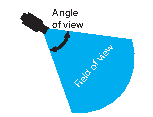
\includegraphics[width=\textwidth]{gfx/camera_properties.pdf}
    \caption{A cameras field of view}
    \label{fig:camera_properties}
\end{figure}

An environment can contain physical objects which limits the cameras field of view further, see Figure~\ref{fig:refular_camera_setup}.
In small environment a sufficient degree surveillance can be achieved without too much difficulty or cost\fixme{Statement - source til prisetr evt.}.
Properly surveilling large areas, in particular outdoor changing environments, is however problematic.\fixme{ref til Lytzen}

\subsection{Video Surveillance of large Outdoor Areas}\label{subsec:surveillance_of_large_outdoor_areas}
%The need for video surveillance is based on the need for documentation of crimes, which is required in case of damage loses from an insurance perspective.
%Should a break-in occur a definitive proof of such must often be presented in order for insurances to cover potential losses.
%Similarly video footage or witnesses is in most cases required in order to convict a person of a burglary.
%One solution to the problem is to have mounted video cameras.
Video cameras have a limited field of view, both in terms of vision and range, and only within this field of view is the quality high enough be usable as documentation.
This limitation can make it difficult and resource intensive to surveil large areas.
The resource intensitivity stems from the amount of hardware required to surveil, referring to both cameras, and the cables needed to connect the surveillance system.
The difficulty in surveilling the areas comes from the nature of an outdoor environment.
In terms of surveillance an indoor environment is static, as there is a limited amount of entrances and the interior of the buildings in terms of walls and doors remain the same.
In an outdoor environment the weather has to be taken into account.
The weather can be foggy, rainy, and the sun can blind a camera if it is improperly placed.
These conditions makes video surveillance of outdoor areas difficult.
Both indoors and outdoors does however have some challenges that needs to be faced, such as physical objects being moved around creating blind spots etc.

\subsection{Current solutions}
This section will discuss the current solutions used for video surveillance.
The strengths and weaknesses of each solution will be covered.
The figures referenced in this section show the same area with a different surveillance setup to make them comparable.
\subsubsection{Regular camera solution}
In a regular camera solution mounted cameras are used.
These cameras surveil a limited area, and in order to cover a larger area, multiple cameras are needed.
With multiple cameras multiple areas are surveilled simultaneously.
A limitation with a regular camera setup, is that the cameras are stationary.
This means a cameras field of view can be limited by physical objects.
As an example in Figure~\ref{fig:refular_camera_setup} it can be seen how an object placed in a cameras field of view can create a blind spot in an area normally covered by a camera.
\begin{figure}[htb]
    \centering
    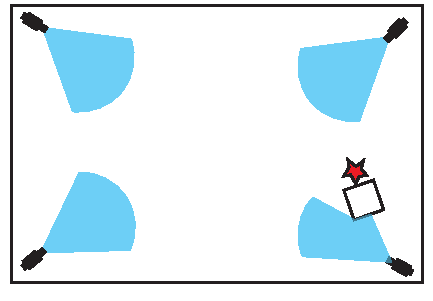
\includegraphics[width=\textwidth]{gfx/regular_camera_setup.pdf}
    \caption{An Example of a Regular Camera Setup}
    \label{fig:refular_camera_setup}
\end{figure}
The red star in Figure ~\ref{fig:refular_camera_setup} represents a critical object, that needs to be observed.

\subsubsection{Photo Sensor Camera Solution}
In a photo sensor solution the perimeter of the surveilled area is covered by both cameras and photo sensors.
The purpose of the setup is to detect if anything enters the area, and then activate the cameras to capture it on video, as seen in Figure~\ref{fig:photo_sensor}.
A photo sensor solution can be used in combination with a regular camera solution, to surveil both the interior and the perimeter of an area.
The advantage of a photo sensor setup is that the cameras surveilling the perimeter are only activated if the sensors are triggered, ensuring video footage is only recorded when it is needed.
The disadvantage is that the cameras are still stationary, meaning the a large amount of cameras are required to surveil a large area.
\begin{figure}[htb]
    \centering
    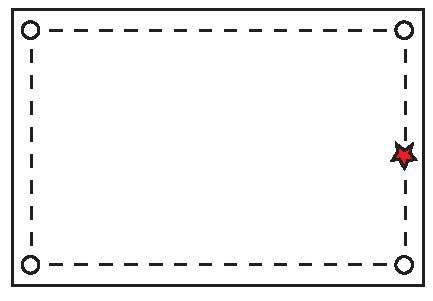
\includegraphics[width=\textwidth]{gfx/light_sensor.pdf}
    \caption{A Photo Sensor Setup}
    \label{fig:photo_sensor}
\end{figure}

\subsubsection{Dome camera solution}
This solution centers around having a dome camera with a long field of view in the center.
The perimeter is then divided into zones, by fx. light sensors.
When a zone have detected an entry, the dome camera is rotated towards that zone to observe the area.
Compared to the two previous solution, the dome camera solution is limited to only observe a specific subarea at a time, as seen in Figure~\ref{fig:drone_sensor}.
\begin{figure}[htb]
    \centering
    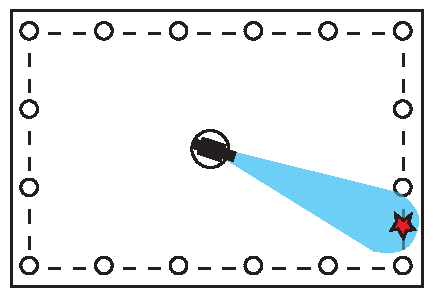
\includegraphics[width=\textwidth]{gfx/drome_sensor.pdf}
    \caption{A Dome Setup}
    \label{fig:drone_sensor}
\end{figure}

\subsection{Moveable Cameras}
As mentioned in Section~\ref{subsec:surveillance_of_large_outdoor_areas} the main problems with surveillance is the ammount of hardware required, particularly cables, and the limited field of view of cameras.
A possible solution is to switch from fixed cameras to movable cameras.
A movable camera is one capable of moving freely in the environment it is to surveil.
This can be achieved with the use of drones with an onboard camera.
A drone in this context is a pilotless aircraft controlled via remote controll.
Drones capable of moving freely in an environment is capable of surveilling a larger area with fewer cameras, than a traditional setup, and they remove the problem with blind spots.
The need for cables is also removed by using drones, as they are typically controlled using wireless internet technologies or radio waves\fixme{source}.

\subsection{Internet Technologies in a Surveillance Perspective}
With the development and standardization of network technologies, video surveillance is becoming digitized.
The digitization of video surveillance is important as it e.g. makes it faster to examine a video recording, and video cameras can be programmed to trigger alarms when they detect movement.
Video recordings are examined faster as it is easy to skip through digital data compared to the analog data which would be stored on e.g. a VHS cassette.
The programming of video cameras is possible due to the data being digital. 
It is possible to apply algorithms to examine the digital Sdata, which could e.g. identify license plates.
The digitization allows for the use of the internet.
The internet makes it possible to interconnect surveillance solution, that enables features such as backup or long distance observing.








%In their current form most security systems consist of a set of sensors and cameras, each covering a limited area.
%Both a sensor and a camera is limited by its range and spectrum.
%As a consequence security systems require a large amount of hardware to monitor a large area to a satisfying degree.
%Hardware is expensive and therefore the cost of....
%However such a surveillance system still suffer from most of its hardware components being static.
%This means that if a sensor is triggered in an area not covered by a camera, a security company would have to send a guard to the location to investigate the source of the alarm.
%The static nature of security systems combined with the high costs security guards makes it very expensive for a company to properly secure their property.\footnote{Sources for this section, pretty important}

%A possible solution to the high cost and static nature of security systems could be a non-static and self movable surveillance system where cameras are placed on a drone capable of flight.
%In such a system a guard would be able to access and control a drone through a web application to investigate what triggered an alarm, and based on a video stream determine whether or not to send someone to the location.
%Moveable cameras would reduce the amount of hardware required, and the manpower required to investigate alarms.
%Therefore the idea of a drone-based surveillance system is interesting to investigate.

%\subsection{}

%The goal of this project is to develop a drone-based surveillance system, in order to reduce economical cost and save manpower.


%Old: static (Both in terms of camereas and possibly the controlcenter), expensive, slow in response (Regular alarm systems).

%New: dynamic, controllable from a single source, possibly cheaper
\section{Problem Definition}
Video surveillance is static and as a concesequence a large amount of hardware is required to properly surveil an area.
This is problematic when a large area has to be survailed, as it requires a lot of hardware.
Drone technology offers a possible solution to this problem by making video surveillance dynamic through moveable cameras.
This possible solution yields the following preliminary problem statement:\\

\textit{How can drone technology be applied in a software application to improve the effeciency of video surveillance?}\\

From the preliminary problem statement the following aspects must be considered:
\begin{itemize}
	\item How to control a drone through the web application
	\item How to provide video streaming of the drones camera through the web application
	\item How to make the web application scalable to support more than one drone
	\item How the make the system accesible from remote locations in a secure manner
\end{itemize}



\footnote{SKAL RETTES TIL EFTER SAMTALE MED VAGTFIRMA, pr�ver bare at f� defineret et cirka problem}

\section{Problem Statement}


\section{System Definition}
\projectname{} is a web service for multi drone-based surveillance. It allows a user to access and control a drone. The drone is controlled through keyboard gestures with a streamed video feed providing visual information about the drone’s physical environment. \projectname{} connects the user to a physical drone, through their browser. Before a connection is established the user is authenticated in order to provide security features.
\chapter{Analysis}
\section{Problem Domain}
\label{sec:problem_domain}

%\fxfatal{Mangler: Der skal v�re minimum delay p� streamen / video feed da dette g�r det nemmere at styre dronen. - nej, det her er analysen! /a}


%Hvilke overvejelser skal der g�res omkring den wireless connection
%Hvilke overvejelser skal der g�res omkring at gemme videoen ned
%Hvilke overvejelser skal der g�res jurisik i forhold til overv�gning
%Hvilke overvejelser skal der g�res omkring sikkerhed i systemet og person f�lsom data
%Hvad er hovedpunkterne i problem domain
%Hvilke krav stiller de til l�sningen

The problem domain for the application is video surveillance of large outdoor areas.
The solution investigated in this report is to handle this using a drone with a camera instead of stationary cameras.
The solution is intended to be used commercially by different businesses that may each have several different areas or locations that needs to be surveilled.\\

Video surveillance using drones has a set of challenges which must be considered.
In order to ensure that the drone performs the commands that it is sent, the connection to the drone have to be reliable.
%In order to ensure that the drone reacts to the commands that it receives, it is required to have reliable connection
If the connection to the drone is lost the drone might crash, which must be avoided.
The large outdoor areas require that the connection is stable at long range.
Additionally the connection must support interaction with other services, making it possible to remotely control the drone using the web application as proposed in the problem statement.
Furthermore the system must be scalable to include several locations, meaning several drones, and users simultaneously. \\

For video surveillance to be usable as documentation the video must be stored.
It can be stored directly on the drone, or it can be stored externally.
Storing it on the drone increases the hardware requirements for the drone, as it must be ensured the data is not lost should the drone crash.
The alternative is to stream the video feed via the connection to the drone and store it externally.
This reduces the requirements to the drone, but increases the requirements to the connection as the video feed must be usable.\\

There are two legal aspects to consider with regards to video surveillance.
Firstly there are laws that limit the areas on which it is allowed to video surveil in Denmark \citep{lov_om_tv_overvaagning}, where this project is developed.
This is not an issue for video surveillance with stationary cameras, as they are simply placed in locations that ensure they do not violate these laws.
With movable cameras it needs to be ensured the video surveillance is done within the given laws. 
Furthermore the system must be secure.
In this context secure means that access to the sensitive information is restricted, both internally and externally\\

 
The problems present in the problem domain are therefore as follows:\\
\begin{itemize}
	\item Wireless short-distance (with the drone, see Appendix~\ref{app:ar_drone_specification}) and wired long-distance communication (back to the user) with a drone. This includes controlling the drone.
	%We know that a drone will be near an area that it shall survival, and that the operator might be located far away. Therefore it is necessary that the system can communicate over long distances. 
	\item Wireless short-distance and wired long-distance video streaming. The drone must be able to send back the video feed from its cameras. Therefore the system must also be able to transmit a video feed in real-time over long distances.
	%\item Interaction with the drone will be handled through a web application. It is already decided that the user must be able to control the drone via a web application. Therefore we need to look into how one can do this, knowing that the web is a state-less environment. 
	\item Permissions- and access control in the web application. This includes both access to the system and access to specific drones.
	\item Scalability - the system must be scalable in terms of users and drones.
\end{itemize}

From these problems a set of requirements for \projectname{} can be derived:\\

\begin{itemize}
	\item A user must be able to login to the system.
	\item The system must have security measures in place to make sure any user only sees what he is permitted to.
	\item A drone must be able to send its video feed to the web application, as proposed in the problem statement.
	\item A drone must be controllable from the web application, as proposed in the problem statement.
	\item The system must support multiple drones and users.
\end{itemize}

A set of use cases have been derived from these requirements.
\section{Requirements}
The superficial requirements of \projectname{} are:

\begin{itemize}
	\item A user must be able to log in to the system.
	\item The system must have security measures in place to make sure any user only sees what he is permitted to. 
	\item A drone must be able to send its video feed to the web service.
	\item A drone must be controllable from the web service. 
	\item The system must support multiple drones and users. 
\end{itemize}

These requirements are the base line for the use cases, which will be used to define the final requirements of the system. 

\section{Use cases}
The functionality of the system will be defined through use cases, describing how a user of the system would desire to interact with the system.
The use cases are derived from the requirements described in Section~\ref{sec:problem_domain}.
The use cases can be seen in Table~\ref{tab:use_cases}.\\

\begin{figure}[H]
\begin{center}
\begin{tabular}{ | l | p{6cm} | }
  \hline              
	\textbf{ID} & \textbf{User Case} \\ \hline
	%%%%%%%%%%%      %%%%%%%%%%%S
	%%%%%%%%%%% OBS! %%%%%%%%%%%
	%%%%%%%%%%%      %%%%%%%%%%%
	% Inden tallene �ndres, skal der lige gøres opmærksom på det, da de bruges andre steder.
	1 & As a user I want to be able to login into the system.\\ \hline
	2 & As a user, when I am logged in, I want content shown based on my privileges. \\ \hline
	3 & As a user I want to pilot a specific drone.\\ \hline
	4 & As a user I want to view the video feed of a specific drone. \\ \hline
	5 & As a user I want to be able to grant or revoke other users the privileges that I am an admin of. \\ \hline
	6 & As a user with rights I want to change the settings for a specific drone. \\ \hline
	7 & As a user I want to be able to add and remove a drone to a company. \\ \hline
	8 & As a user I want an overview of all drones my privileges grant me access to.\\ \hline
	9 & As a user I want to be able to log out.  \\ \hline
	10 & As a user with rights I want to be able to create and edit users.  \\ \hline
	11 & As a user with rights I want to be able to create a new company.  \\ \hline
	12 & As an owner of a company, I want to be able to edit the company.  \\ \hline
	13 & As a user I want to be able to edit privileges, that I am allowed to edit, for another user.  \\ \hline
	14 & As a user I want to be able to become a customer.  \\ \hline
	15 & As a user I want to be able to add and remove privileges from a role that i am an admin of.  \\ \hline
	16 & As a user I want to be able to add roles to users within the company I am allowed to do so.  \\ 
  \hline  
\end{tabular}
\caption{Use Cases}
\label{tab:use_cases}
\end{center}
\end{figure}

The use cases define a set of objects which must be present in \projectname{} in order for the use cases to be implementable.
The objects reflect elements in the problem domain which must be modelled in the system.
The objects are \textit{users}, \textit{drones}, \textit{companies}, \textit{roles}, and \textit{privileges}.
Everybody using \projectname{} are classified as \textit{users}, including customers, owners of companies, system admins etc.
However as reflected in the use cases \textit{users} will not have unrestricted access to the system.
Access to the system will be restricted through \textit{privileges}.
As defined in use case \#8 privileges grants access to functionality, meaning a \textit{user} will not have access to anything by default.
A \textit{drone} refer to a physical drone.
\textit{Companies} is used as a grouping of associated \textit{users}, \textit{drones}, and \textit{roles}.
As an example a company might purchase a set of drones for surveilling their property.
The company would need a set users for its employees, and a set of privileges granting access to its drones.
The \textit{company} object would handle this grouping.
Use case \#15 defines a role as at set of privileges, that can be associated with a \textit{company} and granted to \textit{users}.\\

As video surveillance is concerned with sensitive information, security in \projectname{} is important.
This is reflected in use case \#1 and \#2.
User authentication is used as the user must login to access to the content of system.
Access is then further restricted with \textit{privileges}, as the user's access to content is based on his privileges.
Privileges must therefore be designed to be applicable to all aspect of \projectname{}, and be able to restrict access to all parts of the system.
Restricting users access to certain parts of the system once they have gained entry is however not sufficient security for such a system.
It must also be considered how the system can be made secure from external attacks.



\section{Development Platform}
\section{Development Method}\label{sec:developmet_method}
%P� hvilken baggrund v�lges en udviklingsmetode
%Under hvilke omst�ndigheder udf�res dette projekt
%Hvilke udviklingsmetoder er brugbare baseret p� omst�ndighederne
%Hvilken udviklingsmetode bruges og hvordan er den implementeret i projektet.

%We have had experience with different development methods from previous semesters, more specifically Scrum and XP.
%During these semesters we learned to take advantage of using common Scrum principles such as stand-up meetings, making short and precise iterations and to postpone tasks to the next iteration if not completed.
%We are, however, aware that Scrum might not fit exactly on this project.
%Therefore we have analyzed what is required from this project and how we need to modify Scrum in order to fit to our needs. \\

%We will implement all the principles from Scrum. In addition to this, we have changed and/or added the following to our modified version of Scrum:
%\begin{itemize}
%    \item Pair programming. We have decided to add the principles of pair programming, found in XP, to our project. We are working in an area of great uncertainty, as we have no prior experience with a lot of the problem domain. To lower the number of errors and faster get an understanding of our system, we have decided to implement Pair Programming.
%    \item Refactoring. Also due to the uncertainty of this project, we have added refactoring sessions to our iterations. These are also normally found in XP. They are added to enable us to improve our code over time.
%\end{itemize}

%The reason why we have chosen not to use any of the traditional development methods such as the Waterfall model is that its procedural and locked procedures does not fit a project, where the problem domain contains a lot of uncertainties and unknown areas. We need to be able to look back at what we have done and learned in the previous iterations, refactor, re-design, improve and re-implement parts of the solution. Our modified version of SCRUM allows us to accomplish this.



The choice of development method is based on previous experience and which method best suits the project.
Which development method best suits a project is determined by the circumstances under which it is being done.
The project is being done by a fixed size group of five members with a hard deadline.
All participants in the project have similar experience with software development methods, both agile and traditional methods.
The problem domain for the project is well defined, as there are no uncertainties in regards to the required functionality of the system.
The functionality defined by use cases does however contain unknown such as video streaming, a distributed system, and communication with a drone.
These unknown subjects creates an uncertainty about how to implement the desired functionality.
Other factors to consider is the participants motivation, which can be affected by the chosen development method.\\

From the circumstances it can be derived that a traditional development does not fit the project.
As the solution domain is unknown, creating a large upfront design is undesirable and might not be possible.
Furthermore the hard deadline means that with a traditional method there is the risk that very little, or even none of the functionality is implemented, as the design phase might become to long or complex due to the uncertanties in the solution domain.\\

Therefore the best suit for this project is an agile development method.
The usefull aspect of the agile development methods is their iterative nature.
An iteretive development method allows for refactoring, redesign, and most importantly for this project, the possibility of not implementing some functionality to meet the hard deadline.
The agile development methods considered for this project are Extreme Programming \textit{(XP)} and Scrum.\\

Both development methods have practices usefull for the project.
Therefore the development process for the project is a combination of the two.
The practises taken from Scrum are:
\begin{itemize}
	\item Sprint planning meetings
	\item A Sprint backlog of the tasks for the current spring
	\item Daily stand-up meetings
\end{itemize} 

The practices taken from XP are:
\begin{itemize}
	\item Pair-programming
	\item Acceptance tests
\end{itemize}
\section{AR Drone 2.0 Parrot}

Hvad er det? Beskrivelse af dens teknik, styresystem, hvordan den selv broadcaster et wifi mv.

\chapter{Architecture}

This chapter will describe the architecture of the software that is built in this project.

% Beskriv hvilke valg der ligger til grund for designet af vores model
% hvad lægger vi vægt på? 
% Koncentet med en drone, en slave og en master - skalérbarhed
% Brugere, rettigheder, permissions osv.


\section{Idea}
We want an architecture that supports three things:

\begin{itemize}
	\item Drone and User interaction
	\item Different access to the system on a per user basis 
	\item Scalability in regard to both usage and the scope of the system
\end{itemize}

These architectural goals are a mixture of the requirements of this project and the needs described in the analysis. 
They will be described in the following. 


\subsection{Drone and User interaction}
A User should be able to interact with a Drone via the system.
This includes both watching the video feed and controlling the Drones movements.
This is one of the most important features in the system.
Therefore it is important the the systems architecture supports it natively. 


\subsection{Different access to the system on a per user basis}
Another important feature is support of multiple users and drones, and not least support of different access level for different users.
Not all users should be able to see all drones, and therefore some security/access system needs to be implemented into the model. 


\subsection{Scalability in regard to both usage and the scope of the system}
The security/access system makes sure that the system is scalable in regard to adding more users or drones. 
But the architecture must also make sure that the system does not only scale up, but also out. 
There may come a point where the system needs to support other objects than drones, such as stationary cameras or other equipment. 
In that situation the system needs to be able to handle this without needing to change the source code first.
Therefore, this must be a part of the architecture already now. 


\subsection{Communication between a Drone and the web service}
Since the AR Drones are broadcasting their own WIFI network that one can connect to, instead of being able to connect to an existing WIFI network, them implementation is sort of backwards. 
This means that the Drone is not able to connect directly to the web service. 

\begin{figure}[htb]
    \centering
    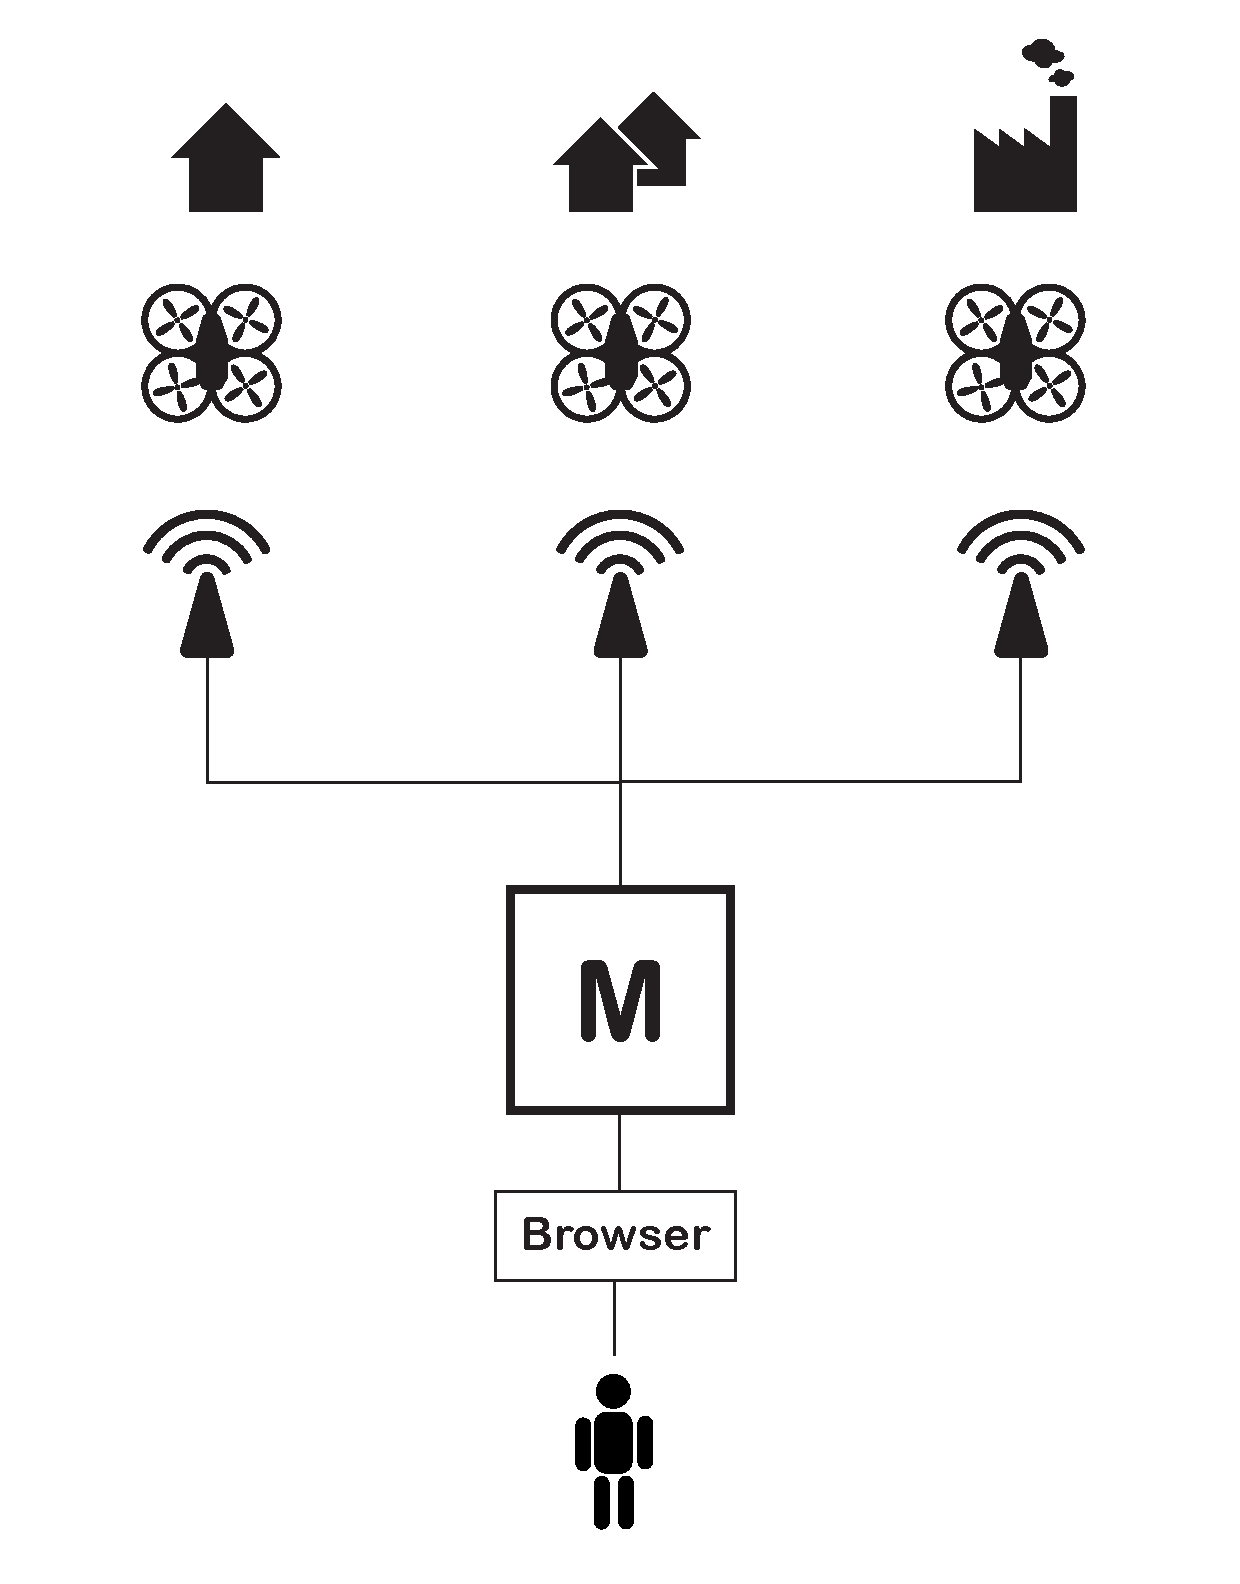
\includegraphics[width=\textwidth]{gfx/technical_structure.pdf}
    \caption{Illustration of the relationship between Drones and the end User}
    \label{fig:Technical_Structure}
\end{figure}

Figure~\ref{fig:Technical_Structure} shows the architecture of the physical elements (drones, servers and users) and is also an example with one user and three drones, each located at three different locations.
Due to the AR Drones nature where they broadcast a WIFI that a client must connect to, each location has a ``Slave''-server that connects to a Drones WIFI. 
Each client then communicates with the ``Master''-server (which is also hosting the web service), which a user can connect to via his Internet Browser. 
That means that the communications flow from the user to the drone will be as displayed in Figure~\ref{fig:Technical_Structure}.

\section{UML notation}

This report will be guided by the UML standard guide written by many respected software firms \citep{UML_notation}.
Because this project uses Active Relations it is possible to model the database as a class diagram. Or in other words the classes in the system will represent the database attributes with their own attributes.

The UML notation in this report:
\begin{itemize}
	\item PK attribute - means that the attribute is a primary key.
	\item FK attribute - means that the attribute is a foreign key.
	\item attribute : type - all attributes will have a type e.g. id : int.
\end{itemize}

\fixme{Not done.}
\input{Chapters/architecture/model}
\section{System architecture}
\begin{figure}[htb]
    \centering
    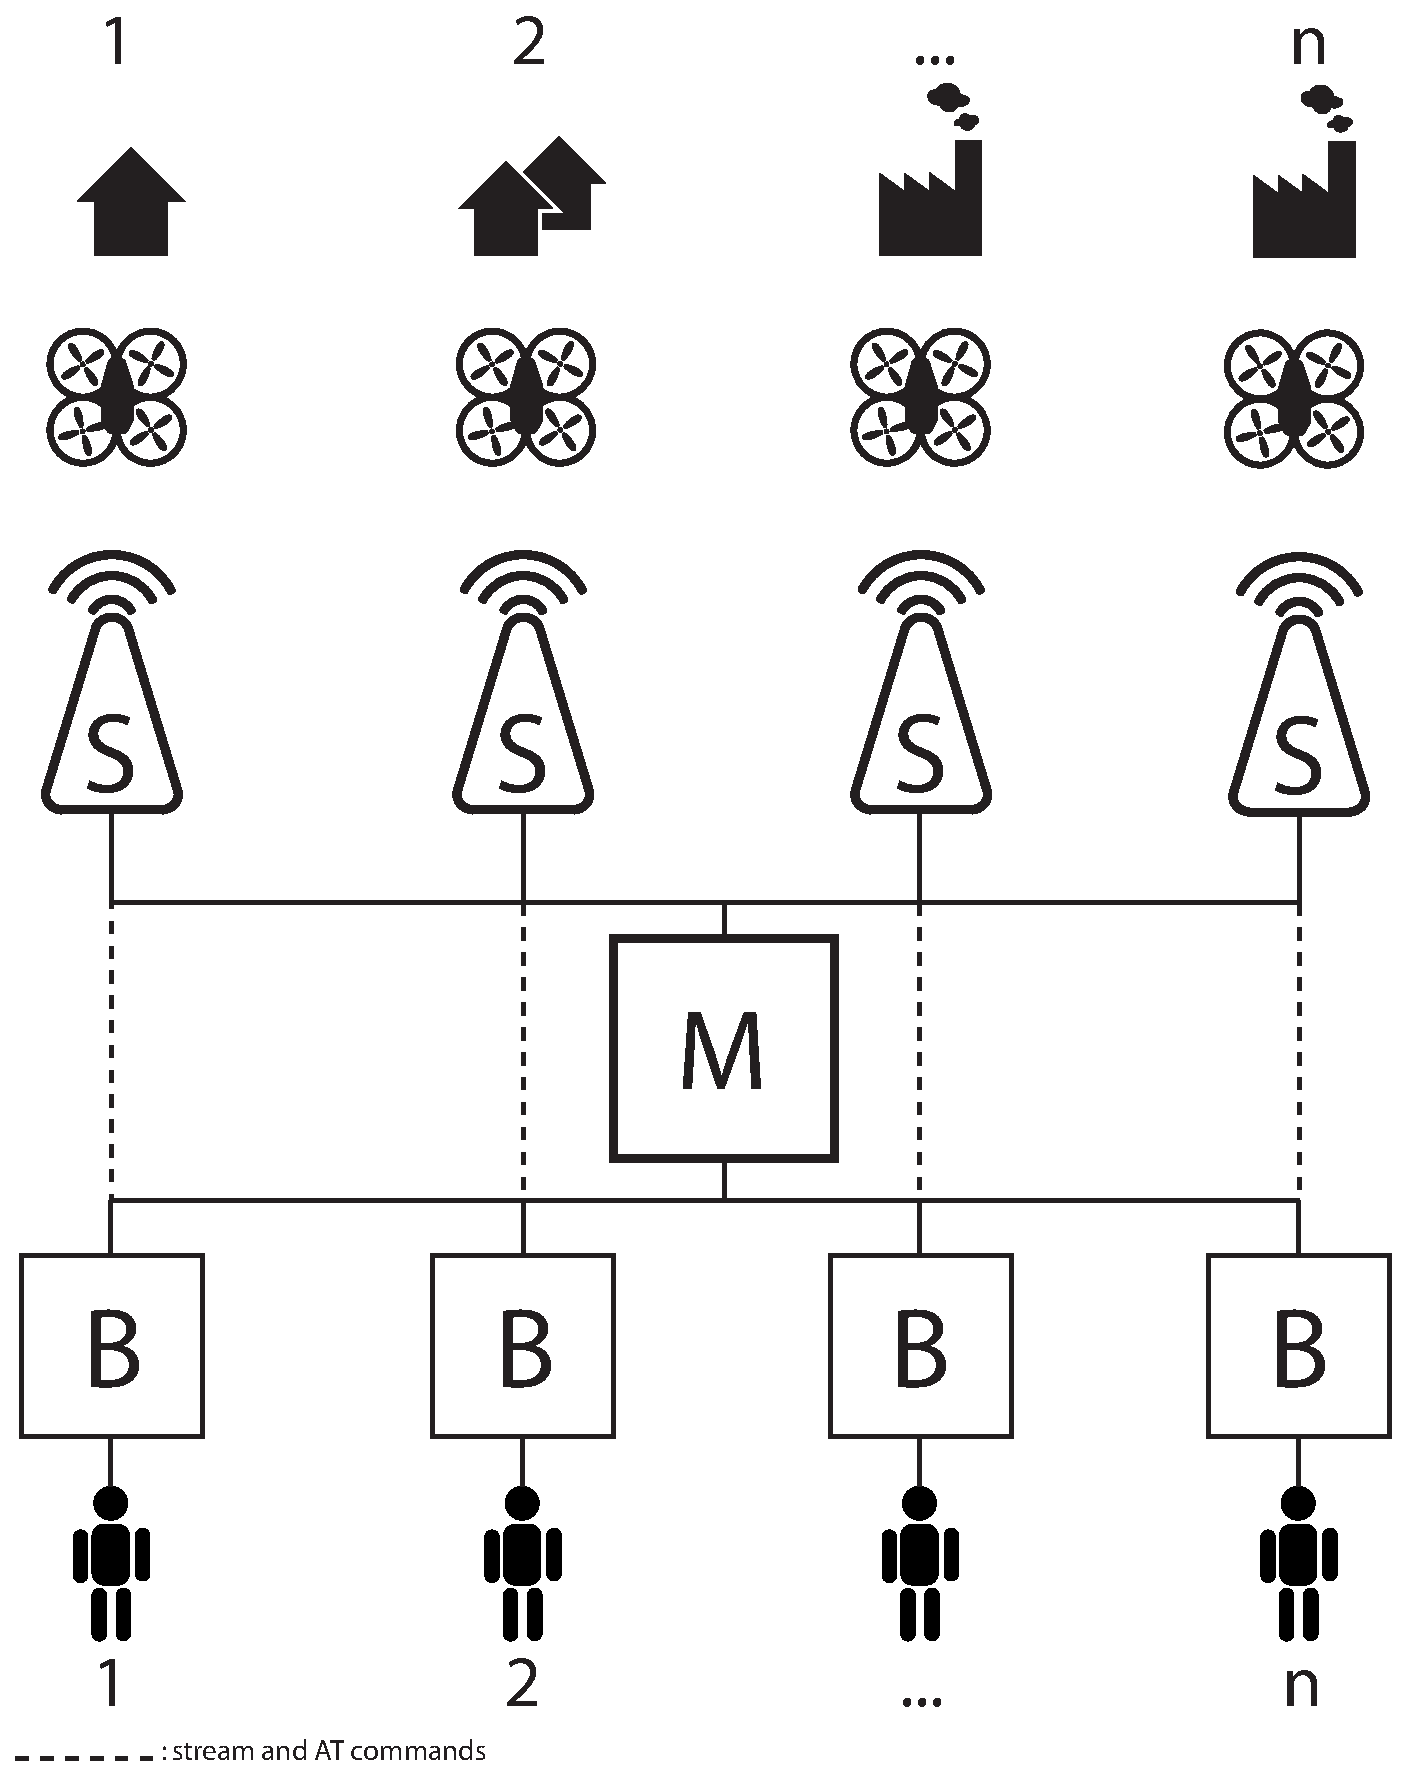
\includegraphics[width=\textwidth]{gfx/system_architecture.pdf}
    \caption{System architecture of \projectname{}}
    \label{fig:system_architecture}
\end{figure}


\chapter{Architecture}

This chapter will describe the architecture of the software that is built in this project.

% Beskriv hvilke valg der ligger til grund for designet af vores model
% hvad lægger vi vægt på? 
% Koncentet med en drone, en slave og en master - skalérbarhed
% Brugere, rettigheder, permissions osv.


\section{Idea}
We want an architecture that supports three things:

\begin{itemize}
	\item Drone and User interaction
	\item Different access to the system on a per user basis 
	\item Scalability in regard to both usage and the scope of the system
\end{itemize}

These architectural goals are a mixture of the requirements of this project and the needs described in the analysis. 
They will be described in the following. 


\subsection{Drone and User interaction}
A User should be able to interact with a Drone via the system.
This includes both watching the video feed and controlling the Drones movements.
This is one of the most important features in the system.
Therefore it is important the the systems architecture supports it natively. 


\subsection{Different access to the system on a per user basis}
Another important feature is support of multiple users and drones, and not least support of different access level for different users.
Not all users should be able to see all drones, and therefore some security/access system needs to be implemented into the model. 


\subsection{Scalability in regard to both usage and the scope of the system}
The security/access system makes sure that the system is scalable in regard to adding more users or drones. 
But the architecture must also make sure that the system does not only scale up, but also out. 
There may come a point where the system needs to support other objects than drones, such as stationary cameras or other equipment. 
In that situation the system needs to be able to handle this without needing to change the source code first.
Therefore, this must be a part of the architecture already now. 


\subsection{Communication between a Drone and the web service}
Since the AR Drones are broadcasting their own WIFI network that one can connect to, instead of being able to connect to an existing WIFI network, them implementation is sort of backwards. 
This means that the Drone is not able to connect directly to the web service. 

\begin{figure}[htb]
    \centering
    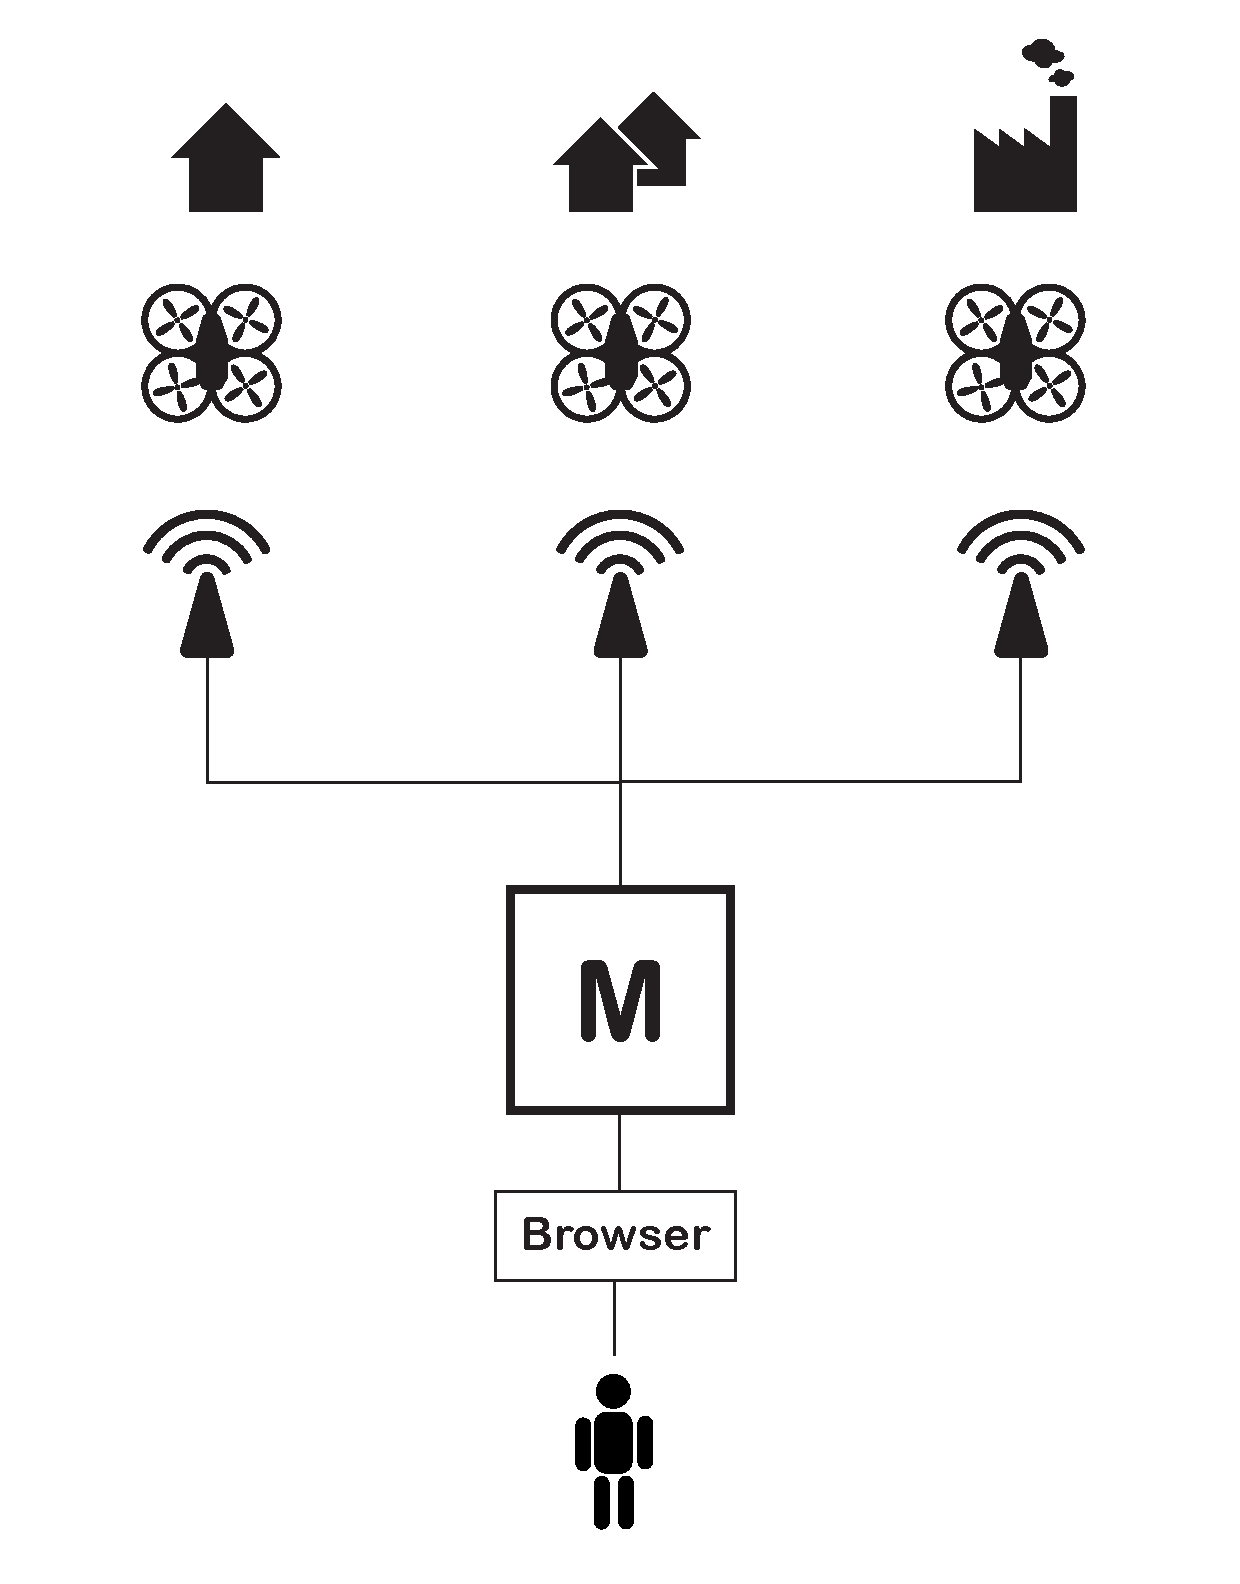
\includegraphics[width=\textwidth]{gfx/technical_structure.pdf}
    \caption{Illustration of the relationship between Drones and the end User}
    \label{fig:Technical_Structure}
\end{figure}

Figure~\ref{fig:Technical_Structure} shows the architecture of the physical elements (drones, servers and users) and is also an example with one user and three drones, each located at three different locations.
Due to the AR Drones nature where they broadcast a WIFI that a client must connect to, each location has a ``Slave''-server that connects to a Drones WIFI. 
Each client then communicates with the ``Master''-server (which is also hosting the web service), which a user can connect to via his Internet Browser. 
That means that the communications flow from the user to the drone will be as displayed in Figure~\ref{fig:Technical_Structure}.

\section{UML notation}

This report will be guided by the UML standard guide written by many respected software firms \citep{UML_notation}.
Because this project uses Active Relations it is possible to model the database as a class diagram. Or in other words the classes in the system will represent the database attributes with their own attributes.

The UML notation in this report:
\begin{itemize}
	\item PK attribute - means that the attribute is a primary key.
	\item FK attribute - means that the attribute is a foreign key.
	\item attribute : type - all attributes will have a type e.g. id : int.
\end{itemize}

\fixme{Not done.}
\input{Chapters/architecture/model}
\section{System architecture}
\begin{figure}[htb]
    \centering
    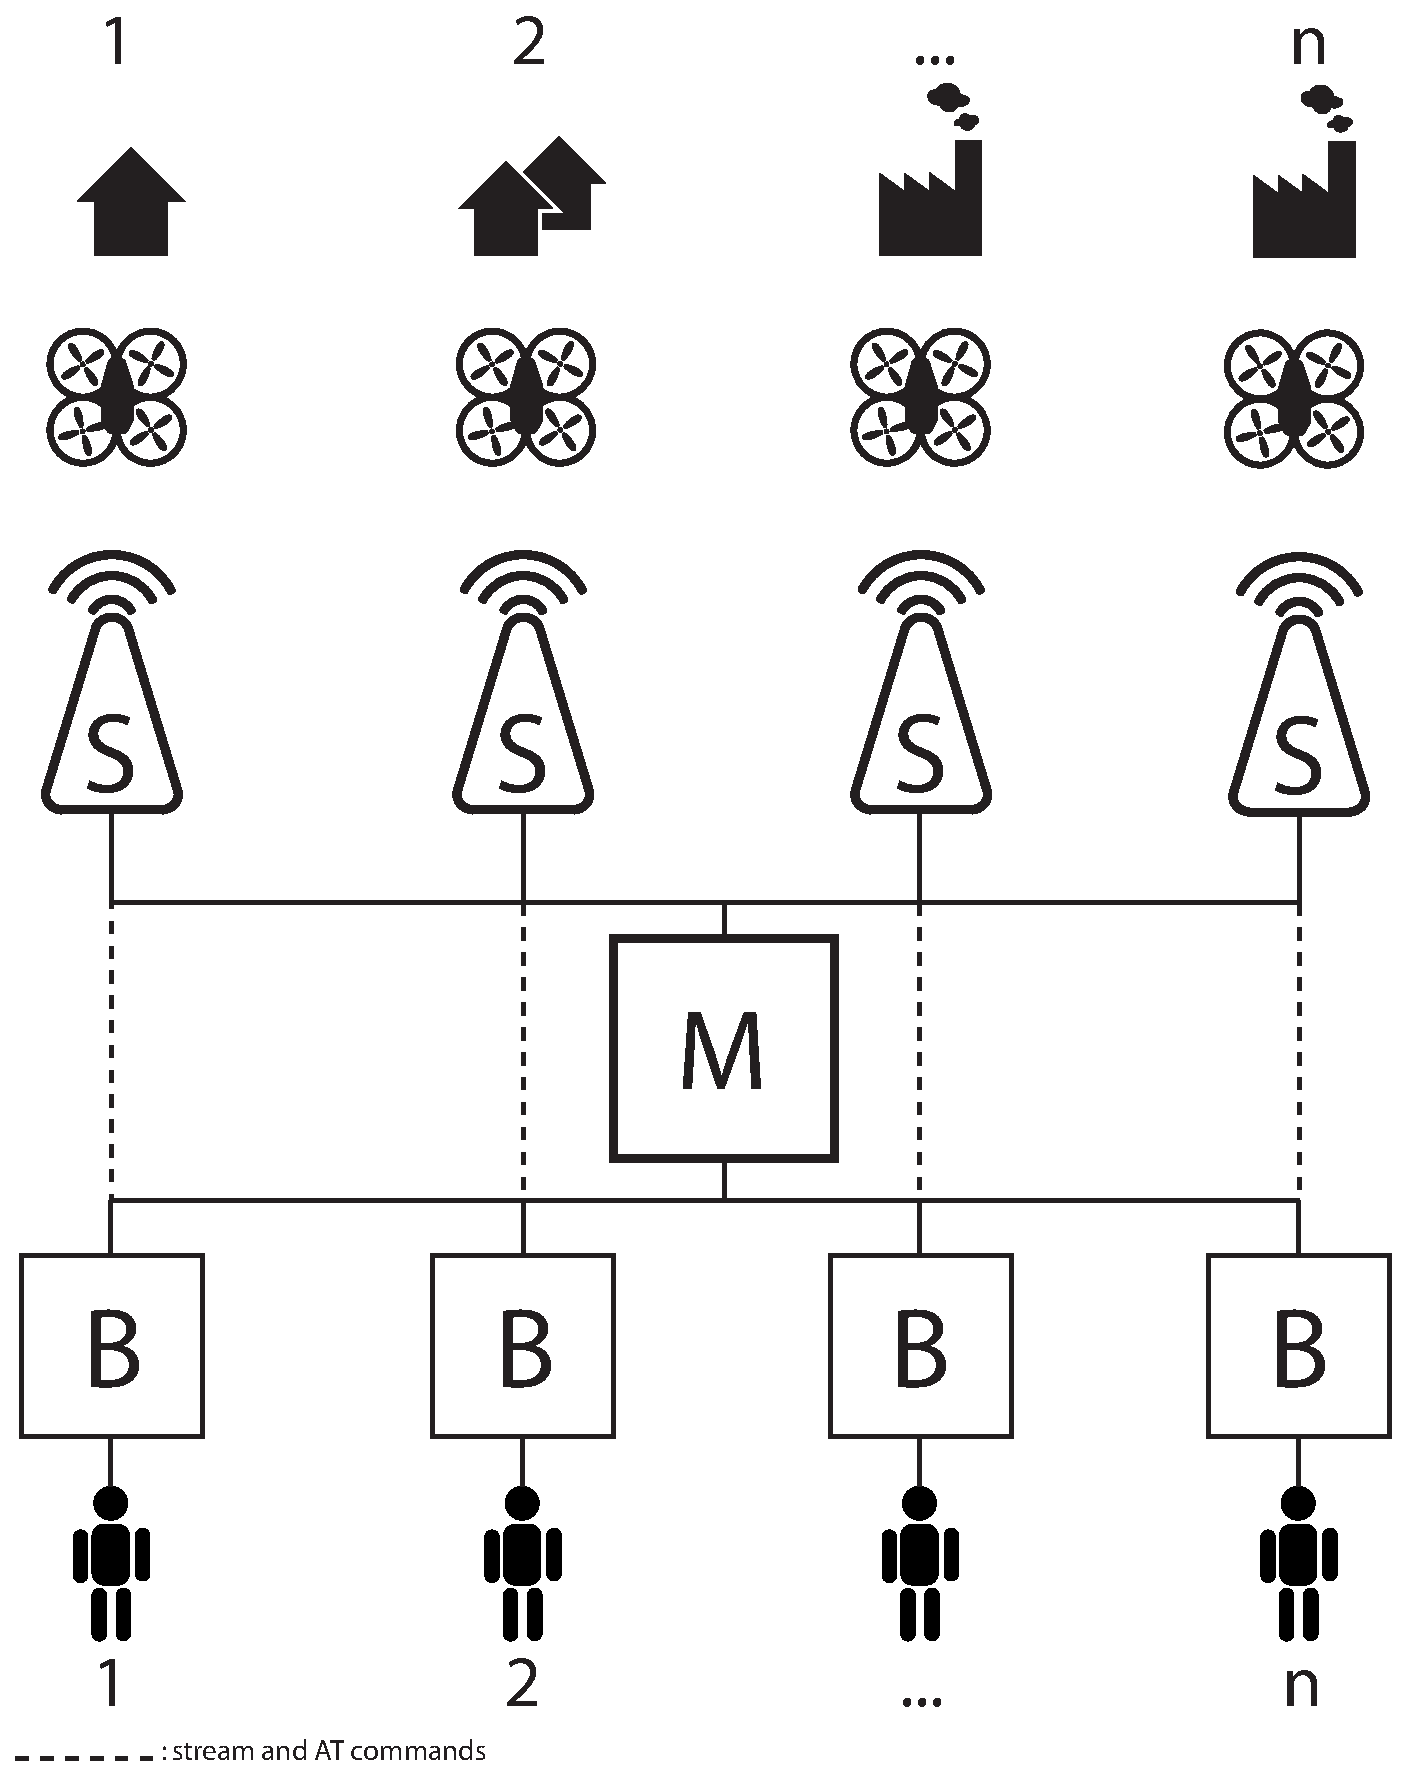
\includegraphics[width=\textwidth]{gfx/system_architecture.pdf}
    \caption{System architecture of \projectname{}}
    \label{fig:system_architecture}
\end{figure}


%\addtocontents{toc}{\protect\clearpage} % <--- just debug stuff, ignore
%%************************************************
\chapter{Math Test Chapter}\label{ch:mathtest} % $\mathbb{ZNR}$
%************************************************
Ei choro aeterno antiopam mea, labitur bonorum pri no. His no decore
nemore graecis. In eos meis nominavi, liber soluta vim cu. Sea commune
suavitate interpretaris eu, vix eu libris efficiantur.

\section{Some Formulas}
Due to the statistical nature of ionisation energy loss, large
fluctuations can occur in the amount of energy deposited by a particle
traversing an absorber element\footnote{Examples taken from Walter
Schmidt's great gallery: \\
\url{http://home.vrweb.de/~was/mathfonts.html}}.  Continuous processes
such as multiple
scattering and energy loss play a relevant role in the longitudinal
and lateral development of electromagnetic and hadronic
showers, and in the case of sampling calorimeters the
measured resolution can be significantly affected by such fluctuations
in their active layers.  The description of ionisation fluctuations is
characterised by the significance parameter $\kappa$, which is
proportional to the ratio of mean energy loss to the maximum allowed
energy transfer in a single collision with an atomic electron:
\graffito{You might get unexpected results using math in chapter or
section heads. Consider the \texttt{pdfspacing} option.}
\begin{equation}
\kappa =\frac{\xi}{E_{\textrm{max}}} %\mathbb{ZNR}
\end{equation}
$E_{\textrm{max}}$ is the maximum transferable energy in a single
collision with an atomic electron.
\[
E_{\textrm{max}} =\frac{2 m_{\textrm{e}} \beta^2\gamma^2 }{1 +
2\gamma m_{\textrm{e}}/m_{\textrm{x}} + \left ( m_{\textrm{e}}
/m_{\textrm{x}}\right)^2}\ ,
\]
where $\gamma = E/m_{\textrm{x}}$, $E$ is energy and
$m_{\textrm{x}}$ the mass of the incident particle,
$\beta^2 = 1 - 1/\gamma^2$ and $m_{\textrm{e}}$ is the electron mass.
$\xi$ comes from the Rutherford scattering cross section
and is defined as:
\begin{eqnarray*} \xi  = \frac{2\pi z^2 e^4 N_{\textrm{Av}} Z \rho
\delta x}{m_{\textrm{e}} \beta^2 c^2 A} =  153.4 \frac{z^2}{\beta^2}
\frac{Z}{A}
  \rho \delta x \quad\textrm{keV},
\end{eqnarray*}
where

\begin{tabular}{ll}
$z$          & charge of the incident particle \\
$N_{\textrm{Av}}$     & Avogadro's number \\
$Z$          & atomic number of the material \\
$A$          & atomic weight of the material \\
$\rho$       & density \\
$ \delta x$  & thickness of the material \\
\end{tabular}

$\kappa$ measures the contribution of the collisions with energy
transfer close to $E_{\textrm{max}}$.  For a given absorber, $\kappa$
tends
towards large values if $\delta x$ is large and/or if $\beta$ is
small.  Likewise, $\kappa$ tends towards zero if $\delta x $ is small
and/or if $\beta$ approaches $1$.

The value of $\kappa$ distinguishes two regimes which occur in the
description of ionisation fluctuations:

\begin{enumerate}
\item A large number of collisions involving the loss of all or most
  of the incident particle energy during the traversal of an absorber.

  As the total energy transfer is composed of a multitude of small
  energy losses, we can apply the central limit theorem and describe
  the fluctuations by a Gaussian distribution.  This case is
  applicable to non-relativistic particles and is described by the
  inequality $\kappa > 10 $ (\ie, when the mean energy loss in the
  absorber is greater than the maximum energy transfer in a single
  collision).

\item Particles traversing thin counters and incident electrons under
  any conditions.

  The relevant inequalities and distributions are $ 0.01 < \kappa < 10
  $,
  Vavilov distribution, and $\kappa < 0.01 $, Landau distribution.
\end{enumerate}


\section{Various Mathematical Examples}
If $n > 2$, the identity
\[
  t[u_1,\dots,u_n] = t\bigl[t[u_1,\dots,u_{n_1}], t[u_2,\dots,u_n]
  \bigr]
\]
defines $t[u_1,\dots,u_n]$ recursively, and it can be shown that the
alternative definition
\[
  t[u_1,\dots,u_n] = t\bigl[t[u_1,u_2],\dots,t[u_{n-1},u_n]\bigr]
\]
gives the same result.  

%*****************************************
%*****************************************
%*****************************************
%*****************************************
%*****************************************

%\include{multiToC} % <--- just debug stuff, ignore for your documents
% ********************************************************************
% Backmatter
%*******************************************************
\appendix
\cleardoublepage
\part{Appendix}
\chapter{Appendix}
\chapter{Interview with Lytzen IT}
\label{appendix:lytzen_it}
The interview were setup with Lytzen IT via email and they were the only alarm company to contact us back. \\

Lytzen IT were presented by both S�ren Ole S�ndergaard and Jesper Toft. S�ren is one of the partners that owns Lytzen IT and Jesper is their alarm and security specialist.
The meeting found place at Lytzen AS and Lytzen IT's headquarters in Hj�rring, Friday the 12 December. \\

In the meeting the project were presented and the idea about drone surveillance. What the thought was and what the system could solve of problems in todays world. 
An example was surveillance of AAU buildings where there are install contacts on every window in this way they can tricker an alarm. The alarm will only go off in a certain time interval of the day if it is a workday and all the time if it is in the weekends. One of the problems is if a student accidently opens a window and the alarm goes of a guard must come and check it out which is very costly. Here the drone could be placed inside the building and flown around to check alarms before sending a guard. \\

Lytzen IT had some cases where they either have used a lot of small cameras or one big dome camera to make a CCTV, Closed-Circuit TeleVision. A dome camera is a camera which can turn 360$^\circ$ and in the big models have a great optic zoom. Because of all these features these dome cameras can surveillance a big area but there is some short comings. They are expensive, they have to be placed high up to be able to see everything and if there are objects they cant see ``behind'' them. For out the cameras being very expensive the cables for these cameras are even more so. They need to be shielded against weather and being in the ground. They need to be laid in a certain depth.
In large outdoor areas the drones are probably more suited than the stationary cameras. They can go almost everywhere and are not as expensive as the big dome camera or a lot of small cameras with all the cables needed. But the drone system presented also have some short comings. Firstly it is using the global Internet. They think as CCTV is a closed-circuit our drone stream and communication should be the same.
Lytzen also pointed out that the station where the drone needs to charge needs to have some technology that ensures the drone can just land and then charge without any human interaction. The ``charge to fly time ratio'' should be better before it can be used in a real case.
Another thing was that the drone maybe should use radio communication instead of WIFI because it would both give a more secure line and make the range of the drone higher. Also they think that the drone should be automated more so it is not dependent on a pilot all the time. But they still thought that it will be the future in 5 to 10 years. Surveillance is about getting evidence for the police, insurance company and keeping the evidence safe. The drone can also have a intimidating effect. This is why they think that drone surveillance is the future.
The last problem that Lytzen pointed out was the law. In Denmark you may not record any public places. This could be troublesome when using a drone. But Lytzen IT thinks this is likely to change as Denmark is moving against a total surveillance society. 
%********************************************************************
% Other Stuff in the Back
%*******************************************************
\cleardoublepage%********************************************************************
% Bibliography
%*******************************************************
% work-around to have small caps also here in the headline
\manualmark
\markboth{\spacedlowsmallcaps{\bibname}}{\spacedlowsmallcaps{\bibname}} % work-around to have small caps also
%\phantomsection 
\refstepcounter{dummy}
\addtocontents{toc}{\protect\vspace{\beforebibskip}} % to have the bib a bit from the rest in the toc
\addcontentsline{toc}{chapter}{\tocEntry{\bibname}}
\bibliographystyle{plainnat}
\label{app:bibliography} 
\bibliography{Bibliography}
\cleardoublepage\pagestyle{empty}

\hfill

\vfill


\pdfbookmark[0]{Colophon}{colophon}
\section*{Colophon}
This document was typeset using the typographical look-and-feel \texttt{classicthesis} developed by Andr\'e Miede. 
The style was inspired by Robert Bringhurst's seminal book on typography ``\emph{The Elements of Typographic Style}''. 
\texttt{classicthesis} is available for both \LaTeX\ and \mLyX: 
\begin{center}
\url{http://code.google.com/p/classicthesis/}
\end{center}
Happy users of \texttt{classicthesis} usually send a real postcard to the author, a collection of postcards received so far is featured here: 
\begin{center}
\url{http://postcards.miede.de/}
\end{center}
 
\bigskip

\noindent\finalVersionString

%Hermann Zapf's \emph{Palatino} and \emph{Euler} type faces (Type~1 PostScript fonts \emph{URW
%Palladio L} and \emph{FPL}) are used. The ``typewriter'' text is typeset in \emph{Bera Mono}, 
%originally developed by Bitstream, Inc. as ``Bitstream Vera''. (Type~1 PostScript fonts were made 
%available by Malte Rosenau and
%Ulrich Dirr.)

%\paragraph{note:} The custom size of the textblock was calculated
%using the directions given by Mr. Bringhurst (pages 26--29 and
%175/176). 10~pt Palatino needs  133.21~pt for the string
%``abcdefghijklmnopqrstuvwxyz''. This yields a good line length between
%24--26~pc (288--312~pt). Using a ``\emph{double square textblock}''
%with a 1:2 ratio this results in a textblock of 312:624~pt (which
%includes the headline in this design). A good alternative would be the
%``\emph{golden section textblock}'' with a ratio of 1:1.62, here
%312:505.44~pt. For comparison, \texttt{DIV9} of the \texttt{typearea}
%package results in a line length of 389~pt (32.4~pc), which is by far
%too long. However, this information will only be of interest for
%hardcore pseudo-typographers like me.%
%
%To make your own calculations, use the following commands and look up
%the corresponding lengths in the book:
%\begin{verbatim}
%    \settowidth{\abcd}{abcdefghijklmnopqrstuvwxyz}
%    \the\abcd\ % prints the value of the length
%\end{verbatim}
%Please see the file \texttt{classicthesis.sty} for some precalculated 
%values for Palatino and Minion.
%
%    \settowidth{\abcd}{abcdefghijklmnopqrstuvwxyz}
%    \the\abcd\ % prints the value of the length





\cleardoublepage%*******************************************************
% Declaration
%*******************************************************
\refstepcounter{dummy}
\pdfbookmark[0]{Declaration}{declaration}
\chapter*{Declaration}
\thispagestyle{empty}
Put your declaration here.
\bigskip
 
\noindent\textit{\myLocation, \myTime}

\smallskip

\begin{flushright}
    \begin{tabular}{m{5cm}}
        \\ \hline
        \centering signature \\
    \end{tabular}
\end{flushright}

% ********************************************************************
% Game Over: Restore, Restart, or Quit?
%*******************************************************
\end{document}
% ********************************************************************
